\documentclass[11pt]{article} % type of the document
\usepackage[english]{babel} % language of all the auto generated text
\usepackage{lmodern} % use a high quality font
\usepackage{listings} % include code snippets
\usepackage{color} % use colors
\usepackage{textcomp} % additional symbols
\usepackage[hyphens]{url} % adds the \url command
\usepackage[hidelinks]{hyperref}
\usepackage{graphicx} % used for graphics stuff
\usepackage{subcaption} % allows adding subfigures
\usepackage{fancyhdr} % header and footer
\usepackage{todonotes} % \todo command
\usepackage{everypage} % run stuff on every page
\usepackage{pdfpages} % include pdf files as figures
\usepackage[noindentafter]{titlesec}
\usepackage{xspace} % add spaces after macros if necessary
\usepackage{amstext} % includes the \text command
\usepackage{booktabs} % table styling
\usepackage{lipsum} % lorem ipsum
\usepackage{enumitem}
\usepackage{float} % absolute positioning of floats
\usepackage{amsfonts} % additional fonts (used for \textbb
\usepackage{booktabs} % table styling
\usepackage{longtable} % repeat table header on each page
\usepackage{xspace} % used to correct spacing after abbreviations
\usepackage{amssymb,array}
\usepackage{enumitem}
\usepackage{geometry} % define the geometry of the page
\geometry{a4paper,left=25mm,right=25mm, top=28mm, bottom=28mm} 

\setcounter{tocdepth}{5} % define the depth of the table of contents
\setcounter{secnumdepth}{5} % define the depth of the section structure

% paragraphs look like subsubsubsections
\titleformat{\paragraph}[hang]{\bf}{\thetitle\quad}{0pt}{}
\titlespacing{\paragraph}{0pt}{1em}{0.5em} 

% subparagraphs look like paragraphs used to look
\titleformat{\subparagraph}[runin]{\bf}{}{0.5em}{}
\titlespacing{\subparagraph}{0pt}{1em}{1em}

\newcommand{\Ra}{\ensuremath{\Rightarrow}\xspace}
\newcommand{\ra}{\ensuremath{\rightarrow}\xspace}

\definecolor{dark-gray}{gray}{0.3}

\newcommand{\floatright}[1]{\hfill \textcolor{dark-gray}{#1}}

% adds a foot rule to every page
\AddEverypageHook
{
    \renewcommand{\footrulewidth}{0.4pt}
}

% define escape characters for latex commands in listings
\lstset{%
  escapeinside={(*}{*)},%
}

% define symbols for optional and non-optional properties
\newcommand{\nonoptional}{\ensuremath{{}^{\textbf{\circ}}}}
\newcommand{\nonoptionalif}{\ensuremath{{}^{\textbf{*}}}}

% define minipage in tabular
\newcommand{\cellwrap}[1]{\begin{minipage}[t]{1.0\columnwidth}#1\end{minipage}}

% define abbreviations properly
\newcommand*{\eg}{e.g.\@\xspace}
\newcommand*{\ie}{i.e.\@\xspace}

\newcommand{\pipe}{\ensuremath{|}\xspace}

% define colored text method
\newcommand{\coloredtext}[1]{\color[HTML]{#1}{\##1}}

%%%%%%%%%% DEFINE VARIABLES HERE %%%%%%%%%%%%%%%
\newcommand{\instanceStuff}{\texttt{instance-stuff}}


%%%%%%%%%% TIKZ DEFINITIONS %%%%%%%%%%%%
\newcounter{treeline}

\newcommand{\treeroot}[1]{% Title
	\node[above] at (0,0) {#1};%
	\setcounter{treeline}{0}
}

\newcommand{\folder}[2]{% Title, Level
	\draw[->] (#2-1,-\value{treeline}/2) -- (#2-1,-\value{treeline}/2-0.5) -- (#2+0.5,-\value{treeline}/2-0.5) node[anchor=base,inner sep=0,right] (x) 
      {
\includegraphics[height=.5cm]{img/misc/folder.pdf}} node[anchor=west] at(\tikzlastnode.east) {#1} ;

    \foreach \x in {1,...,#2}
	{
		\draw (\x-1,-\value{treeline}/2) -- (\x-1,-\value{treeline}/2-0.5);
	}
	\stepcounter{treeline};
}

\newcommand{\file}[2]{% Title, Level
	\draw[->] (#2-1,-\value{treeline}/2) -- (#2-1,-\value{treeline}/2-0.5) -- (#2+0.5,-\value{treeline}/2-0.5) node[anchor=base,inner sep=0,right] (x) 
      {
\includegraphics[height=.45cm]{img/misc/file.pdf}} node[anchor=west] at(\tikzlastnode.east) {#1} ;
	\foreach \x in {1,...,#2}
	{
		\draw (\x-1,-\value{treeline}/2) -- (\x-1,-\value{treeline}/2-0.5);
	}
	\stepcounter{treeline};
}

\newcommand*{\vcenteredhbox}[1]{\begingroup\setbox0=\hbox{#1}\parbox{\wd0}{\box0}\endgroup}

% style the header and footer
\pagestyle{fancy}
\fancyfoot[R]{\thepage}
\fancyhead[L]{Germinate 3}
\fancyhead[R]{\nouppercase{\leftmark}\cfoot{}}

\hypersetup{
	pdfauthor={Sebastian Raubach},
	pdftitle={Germinate 3 Documentation},
	pdfinfo={Copyright={Copyright 2013-2017 The James Hutton Institute. All rights reserved.}}
}

\makeatletter
\lst@CCPutMacro\lst@ProcessOther {"2D}{\lst@ttfamily{-{}}{-{}}}
\@empty\z@\@empty
\makeatother

% the document starts here
\begin{document}

% remove page numbers for title and TOC
\pagenumbering{gobble}
% title page is compiled by itself
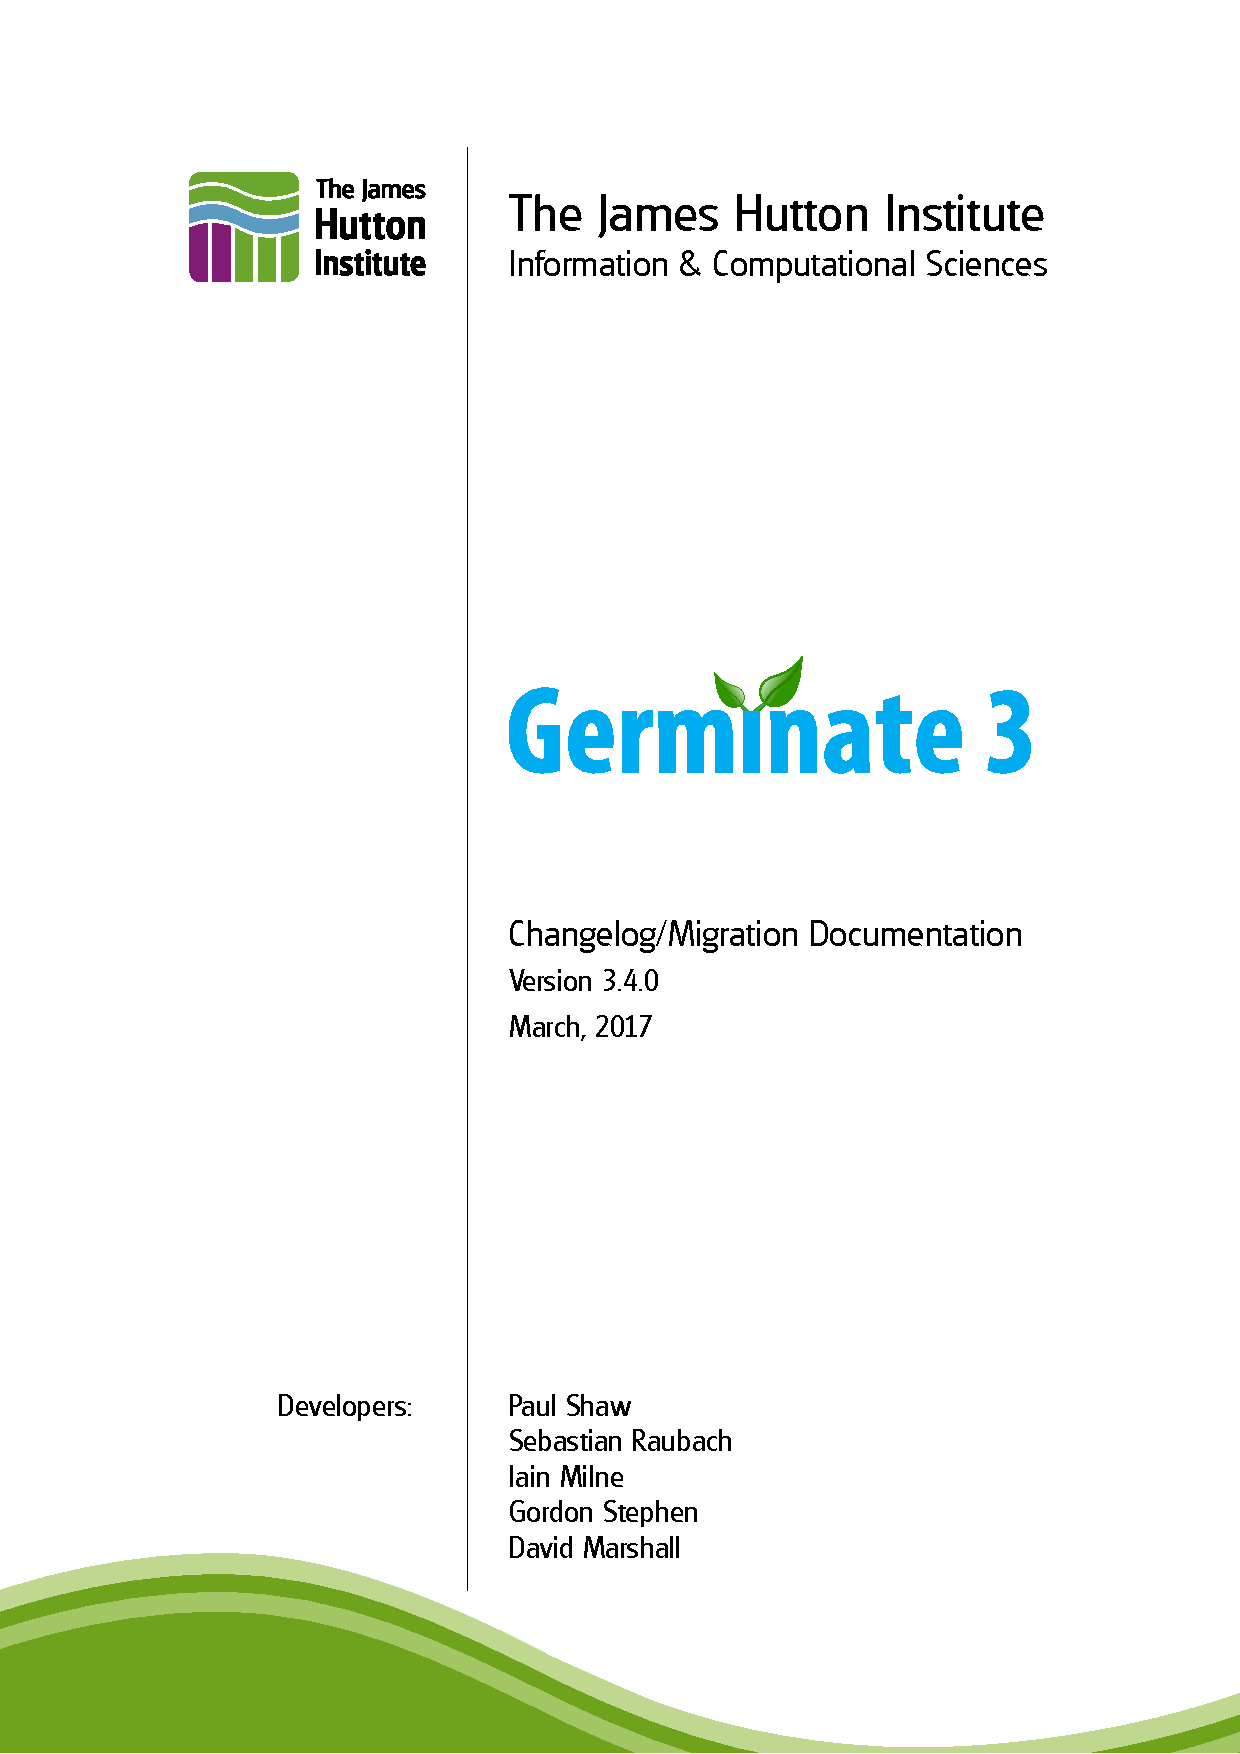
\includepdf{title.pdf}

% add the table of contents
\tableofcontents

% Include the styling of the code snippets
%\include{theme-dark}
% code styling for java
\lstdefinestyle{Java}{
	backgroundcolor=\color[RGB]{240,240,240},
	tabsize=4,
	rulecolor=\color[RGB]{200,200,200},
    frame=tblr,
    framerule=0.1pt,
    framexleftmargin=0pt,
	language=java,
    basicstyle=\scriptsize\color[rgb]{0,0,0},
    upquote=true,
    aboveskip={0.5\baselineskip},
    columns=fullflexible,
    showstringspaces=false,
    extendedchars=true,
    breaklines=true,
    prebreak=,
    showtabs=false,
    showspaces=false,
    showstringspaces=false,
    identifierstyle=\ttfamily,
    keywordstyle=\color[RGB]{32,96,160},
    commentstyle=\color[RGB]{70,70,70},
    stringstyle=\color[RGB]{0,153,51},
    morekeywords={@Override,@RemoteServiceRelativePath,@PluralCount},
}

% code styling for javascript
\lstdefinestyle{JavaScript}{
	backgroundcolor=\color[RGB]{240,240,240},
	tabsize=4,
	rulecolor=\color[RGB]{200,200,200},
	frame=tblr,
	framerule=0.1pt,
	framexleftmargin=0pt,
	language=,
	basicstyle=\scriptsize\color[rgb]{0,0,0},
	upquote=true,
	aboveskip={0.5\baselineskip},
	columns=fullflexible,
	showstringspaces=false,
	extendedchars=true,
	breaklines=true,
	prebreak=,
	showtabs=false,
	showspaces=false,
	showstringspaces=false,
	identifierstyle=\ttfamily,
	keywordstyle=\color[RGB]{32,96,160},
	commentstyle=\color[RGB]{70,70,70},
	stringstyle=\color[RGB]{0,153,51},
	keywords={typeof, new, true, false, catch, function, return, null, catch, switch, var, if, in, while, do, else, case, break},
	morestring=[b]",
	morestring=[b]'
}



% code styling for HTML
\lstdefinestyle{HTML}{
	backgroundcolor=\color[RGB]{240,240,240},
	tabsize=4,
	rulecolor=\color[RGB]{200,200,200},
    frame=tblr,
    framerule=0.1pt,
    framexleftmargin=0pt,
	language=java,
    basicstyle=\scriptsize\color[rgb]{0,0,0},
    upquote=true,
    aboveskip={0.5\baselineskip},
    columns=fullflexible,
    showstringspaces=false,
    extendedchars=true,
    breaklines=true,
    prebreak=,
    showtabs=false,
    showspaces=false,
    showstringspaces=false,
    identifierstyle=\ttfamily,
    keywordstyle=\color[RGB]{32,96,160},
    commentstyle=\color[RGB]{70,70,70},
    stringstyle=\color[RGB]{0,153,51},
    morekeywords={},
}

% code styling for the .properties files
\lstdefinestyle{Properties}{
	backgroundcolor=\color[RGB]{240,240,240},
	tabsize=4,
	rulecolor=\color[RGB]{200,200,200},
    frame=tblr,
    framerule=0.1pt,
    framexleftmargin=0pt,
	language=,
    basicstyle=\scriptsize\color[rgb]{0,0,0},
    upquote=true,
    aboveskip={0.5\baselineskip},
    columns=fullflexible,
    showstringspaces=false,
    extendedchars=true,
    breaklines=true,
    prebreak=,
    showtabs=false,
    showspaces=false,
    showstringspaces=false,
    identifierstyle=\ttfamily,
    keywordstyle=\color[RGB]{32,96,160},
    commentstyle=\color[RGB]{70,70,70},
    stringstyle=\color[RGB]{0,153,51},
    morekeywords={Germinate,GerminateGatekeeper,Database,Username,Password,Server,Name,UsePort,Port,UseAuthentication,
    Debug,KeepTemporaryFileForHours,Template,VersionName,VersionLink,VersionImage,VersionNumber,Title,DatabaseName,
    TwitterLink,Copyright,Flapjack,Path,CreateProjectMain,AvailablePages,BaseSearchColumn,menuMyFanyPage,iSeeTrees,
    welcomeMessage,LogoMap,BaseTableExternalLink,BaseTableExternalLinkColumn,CollectingsiteTreemapColumn,CookieLifespanMinutes,
    AlleleFreq,MakeHistogram,CreateImage,BinData,Java,R,Gatekeeper,HighlightColor,Menu,GradientTop,GradientBottom,
    CategoricalColors,GradientColors,EmailAddress,ShowHomeOnLogin,BCrypt,Rounds,Registration,Enabled,Needs,Approval,GoogleAnalytics,TrackingId,
    CookieNotifier,UploadSizeLimitMB,Social,ShowFacebook,ShowTwitter,ShowGooglePlus,URL,Server,Logging,IsUnderMaintenance,
    ExternalDataFolder,HideIdColumns,AccessionDisplayColumn,IsReadOnly,Gallery,Images,Per,Page,UseToggleSwitches,Show,Search,Logo,Contains,Link,Show,Parallax,Banner,CustomMenu}
}

\lstdefinestyle{CSS}{
    backgroundcolor=\color[RGB]{240,240,240},
	tabsize=4,
	rulecolor=\color[RGB]{200,200,200},
    frame=tblr,
    framerule=0.1pt,
    framexleftmargin=0pt,
	language=,
    basicstyle=\scriptsize\color[rgb]{0,0,0},
    upquote=true,
    aboveskip={0.5\baselineskip},
    columns=fullflexible,
    showstringspaces=false,
    extendedchars=true,
    breaklines=true,
    prebreak=,
    showtabs=false,
    showspaces=false,
    showstringspaces=false,
    identifierstyle=\ttfamily,
    keywordstyle=\color[RGB]{32,96,160},
    commentstyle=\color[RGB]{70,70,70},
    stringstyle=\color[RGB]{0,153,51},
    morekeywords={accelerator,azimuth,background,background-attachment,
	    background-color,background-image,background-position,
	    background-position-x,background-position-y,background-repeat,
	    behavior,border,border-bottom,border-bottom-color,
	    border-bottom-style,border-bottom-width,border-collapse,
	    border-color,border-left,border-left-color,border-left-style,
	    border-left-width,border-right,border-right-color,
	    border-right-style,border-right-width,border-spacing,
	    border-style,border-top,border-top-color,border-top-style,
	    border-top-width,border-width,bottom,caption-side,clear,
	    clip,color,content,counter-increment,counter-reset,cue,
	    cue-after,cue-before,cursor,direction,display,elevation,
	    empty-cells,filter,float,font,font-family,font-size,
	    font-size-adjust,font-stretch,font-style,font-variant,
	    font-weight,height,ime-mode,include-source,
	    layer-background-color,layer-background-image,layout-flow,
	    layout-grid,layout-grid-char,layout-grid-char-spacing,
	    layout-grid-line,layout-grid-mode,layout-grid-type,left,
	    letter-spacing,line-break,line-height,list-style,
	    list-style-image,list-style-position,list-style-type,margin,
	    margin-bottom,margin-left,margin-right,margin-top,
	    marker-offset,marks,max-height,max-width,min-height,
	    min-width,-moz-binding,-moz-border-radius,
	    -moz-border-radius-topleft,-moz-border-radius-topright,
	    -moz-border-radius-bottomright,-moz-border-radius-bottomleft,
	    -moz-border-top-colors,-moz-border-right-colors,
	    -moz-border-bottom-colors,-moz-border-left-colors,-moz-opacity,
	    -moz-outline,-moz-outline-color,-moz-outline-style,
	    -moz-outline-width,-moz-user-focus,-moz-user-input,
	    -moz-user-modify,-moz-user-select,orphans,outline,
	    outline-color,outline-style,outline-width,overflow,
	    overflow-X,overflow-Y,padding,padding-bottom,padding-left,
	    padding-right,padding-top,page,page-break-after,
	    page-break-before,page-break-inside,pause,pause-after,
	    pause-before,pitch,pitch-range,play-during,position,quotes,
	    -replace,richness,right,ruby-align,ruby-overhang,
	    ruby-position,-set-link-source,size,speak,speak-header,
	    speak-numeral,speak-punctuation,speech-rate,stress,
	    scrollbar-arrow-color,scrollbar-base-color,
	    scrollbar-dark-shadow-color,scrollbar-face-color,
	    scrollbar-highlight-color,scrollbar-shadow-color,
	    scrollbar-3d-light-color,scrollbar-track-color,table-layout,
	    text-align,text-align-last,text-decoration,text-indent,
	    text-justify,text-overflow,text-shadow,text-transform,
	    text-autospace,text-kashida-space,text-underline-position,top,
	    unicode-bidi,-use-link-source,vertical-align,visibility,
	    voice-family,volume,white-space,widows,width,word-break,
	    word-spacing,word-wrap,writing-mode,z-index,zoom},
    morestring=[s]{:}{;},
    alsodigit={-},
    sensitive,
    morecomment=[s]{/*}{*/}
}

% code styling for the Eclipse .properties files
\lstdefinestyle{EclipseProperties}{
	backgroundcolor=\color[RGB]{240,240,240},
	tabsize=4,
	rulecolor=\color[RGB]{200,200,200},
    frame=tblr,
    framerule=0.1pt,
    framexleftmargin=0pt,
	language=,
    basicstyle=\scriptsize\color[rgb]{0,0,0},
    upquote=true,
    aboveskip={0.5\baselineskip},
    columns=fullflexible,
    showstringspaces=false,
    extendedchars=true,
    breaklines=true,
    prebreak=,
    showtabs=false,
    showspaces=false,
    showstringspaces=false,
    identifierstyle=\ttfamily,
    keywordstyle=\color[RGB]{32,96,160},
    commentstyle=\color[RGB]{70,70,70},
    stringstyle=\color[RGB]{0,153,51},
    morekeywords={project,name,root,instance,files,tomcat,manager,url,username,password}
}

% code styling for xml files
\lstdefinestyle{Xml}{
	backgroundcolor=\color[RGB]{240,240,240},
	tabsize=4,
	rulecolor=\color[RGB]{200,200,200},
    frame=tblr,
    framerule=0.1pt,
    framexleftmargin=0pt,
	language=xml,
    basicstyle=\scriptsize\color[rgb]{0,0,0},
    upquote=true,
    aboveskip={0.5\baselineskip},
    columns=fullflexible,
    showstringspaces=false,
    extendedchars=true,
    breaklines=true,
    prebreak=,
    showtabs=false,
    showspaces=false,
    showstringspaces=false,
    identifierstyle=\ttfamily,
    keywordstyle=\color[RGB]{32,96,160},
    commentstyle=\color[RGB]{70,70,70},
    stringstyle=\color[RGB]{0,153,51},
}

% code styling for the .properties files
\lstdefinestyle{Proxy}{
	backgroundcolor=\color[RGB]{240,240,240},
	tabsize=4,
	rulecolor=\color[RGB]{200,200,200},
	frame=tblr,
	framerule=0.1pt,
	framexleftmargin=0pt,
	language=,
	basicstyle=\scriptsize\ttfamily\color[rgb]{0,0,0},
	upquote=true,
	keepspaces=true
	aboveskip={0.5\baselineskip},
	columns=fullflexible,
	showstringspaces=false,
	extendedchars=true,
	breaklines=true,
	prebreak=,
	showtabs=false,
	showspaces=false,
	showstringspaces=false,
	identifierstyle=\ttfamily,
	keywordstyle=\color[RGB]{32,96,160},
	commentstyle=\color[RGB]{70,70,70},
	stringstyle=\color[RGB]{0,153,51}
}

% include all the content files (without file extension)
\section{Introduction}
TEST
\section{Setup}
In this section, we will explain how to get Germinate 3 up and running. First, we will explain the requirements and the necessary steps to deploy a self contained WAR (\textbf{W}eb application \textbf{AR}chive) file. The second part contains a detailed description for the advanced user, where we explain how to deploy the application from the source code.

\subsection{Requirements}
We try to keep the requirements of Germinate 3 as basic as possible. In order to run Germinate 3 you will need to have the following applications available on your server:

\begin{itemize}
	\item \textit{Apache Tomcat} (7.0.28 or above) to run the web application
	\item \textit{Java} (8 or above) to run Apache Tomcat and the Germinate 3 server side code
	\item \textit{MySQL} (or \textit{MariaDB}) (5.6.1 or above) database to hold the data\\
	(if you're using 5.7.5 or above, make sure it's not set to use \texttt{ONLY\textunderscore FULL\textunderscore GROUP\textunderscore BY}).
\end{itemize}
\noindent
If you are planning to compile Germinate 3 from source (required if you do not have \texttt{.war} files) you will also need to have the following applications available on the system you're compiling Germinate 3 on:

\begin{itemize}
	\item \textit{Apache Ant} (1.9.1 or above) to compile to \texttt{.war} files
\end{itemize}
\noindent
Please make sure that you have the required applications installed before continuing.

\subsection{Configuration of Apache Tomcat}
If you already have a Tomcat user account, skip this step.\\
\\
Once Apache Tomcat is installed, you will need to create a user account. This user account will be used to deploy Germinate 3 to Tomcat. To add a user account, open the file \texttt{<Tomcat Directory>/conf/tomcat-users.xml} and add the following line:

\begin{lstlisting}[style=Xml]
<user username="<Username>" password="<Password>" roles="manager-gui,manager-script"/>
\end{lstlisting}
\noindent
Just replace the username and password placeholders with the credentials you want to use. Tomcat needs to be restarted after these two steps.

Remember the username and password, we will need them later.

\subsection{Configuration of MySQL}
\label{sec:mysql-basic}
If you already have a MySQL user account that has permissions to query the Germinate 3 and Germinate Gatekeeper databases, skip this step.\\
\\
After the installation of MySQL, you need to create a user account for Germinate 3, so that the web application can query the database.
Remember the username and password, we will need them later.

Once the user is created, you can grant permissions to the newly created user. It is save to grant this user all available permissions for the Germinate 3 and Germinate Gatekeeper database. The minimal set of required permissions are: \texttt{select}, \texttt{insert}, \texttt{delete}, \texttt{update}, \texttt{create view}, \texttt{create routine} and \texttt{execute}.

\subsection{Basic setup}
In the best case, you already have a compiled version of Germinate 3 and Germinate Gatekeeper in the form of a \texttt{.war} file each as well as their database counterparts in your MySQL installation. 

\begin{figure}
	\centering
	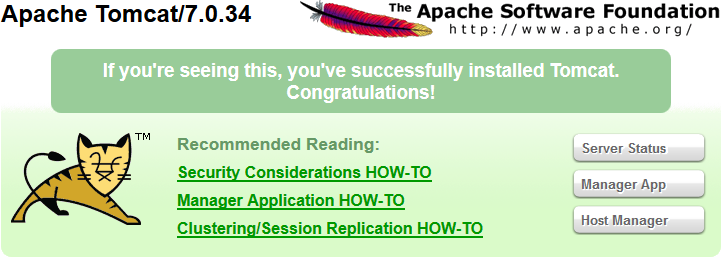
\includegraphics[scale=0.5]{img/setup/tomcat.png}
	\caption{Tomcat welcome screen}
	\label{fig:tomcat}
\end{figure}
\noindent
To deploy these applications, navigate to the following URL:
\begin{center}
	\texttt{http://<Your web server>:8080}
\end{center}
You should see something similar to Figure \ref{fig:tomcat}. Click on the button labelled "Manager App" and you will be prompted to enter your credentials. Use the username and password defined in the file \texttt{tomcat-users.xml}. The following page will show all the applications running on Tomcat right now. Below this table, there is a section called "Deploy" with subsection "WAR file to deploy". Simply select each of the two WAR files by clicking on the "Browse" button and then click on "Deploy". Germinate 3 and Gatekeeper should now be listed in the applications table at the top of the page.

Clicking on the \texttt{Path} link in the first column of the overview table should redirect you to Germinate 3 and Germinate Gatekeeper respectively.

\subsection{Advanced setup}
In this section, we will explain how you compile Germinate 3 (Germinate Gatekeeper analogously) from source. This is required if you do not have pre-compiled versions of the applications. We will also explain how you can create empty versions of the Germinate 3 and Germinate Gatekeeper databases in your database server.

\subsubsection{Download of source code}

First, download the Germinate 3 and Germinate Gatekeeper source code from our SVN:

\begin{itemize}
	\item Germinate 3
	\begin{itemize}
		\item \url{https://ics.hutton.ac.uk/svn/germinate3}
	\end{itemize}
	\item Germinate Gatekeeper
	\begin{itemize}
		\item \url{https://ics.hutton.ac.uk/svn/germinate-gatekeeper}
	\end{itemize}
\end{itemize}

\subsubsection{Configuration of source code}
\label{sec:germinate-config}
Both applications contain a file called \texttt{build.xml} which is the Apache Ant build script as well as an associated \texttt{build.properties} file. These files are used to compile and deploy the application.

Edit the \texttt{build.properties} file and replace the placeholder username and password with your Apache Tomcat username and password. Replace the placeholder for your web server as well.
\begin{lstlisting}[style=EclipseProperties]
# Ant properties for building the GWT app
project.name=germinate-templace
project.root=jhi.germinate.Germinate

instance.files=./(*\instanceStuff*)/template

tomcat.manager.url=http://<Your web server>:8080/manager/text
tomcat.manager.username=<Username>
tomcat.manager.password=<Password>
\end{lstlisting}
\noindent
The next file that needs editing is the \texttt{config.properties} file. In the case of Germinate Gatekeeper this file is located in the root directory. In the case of Germinate 3, you can find this file in the \texttt{\instanceStuff/<your germinate instance>} folder.\\
\\
Configure Germinate Gatekeeper in the following way:

\begin{lstlisting}[style=Properties]
database.server=<server holding germinate>
database.name=<database name>
database.useport=<is a port necessary?>
database.port=<port number>
database.username=<username, e.g. germinate3>
database.password=<password>
[...]
\end{lstlisting}
\noindent
Finally, configure Germinate 3 in the following way:

\begin{lstlisting}[style=Properties]
Germinate.Database.Server=<server holding germinate>
Germinate.Database.Name=<database name>
Germinate.Database.UsePort=<is a port necessary?>
Germinate.Database.Port=<port number>
Germinate.Database.Username=<username, e.g. germinate3>
Germinate.Database.Password=<password>

Gatekeeper.URL=<base url of gatekeeper>
Gatekeeper.Database.Name=<name of gatekeeper database>
Gatekeeper.Database.Server=<server holding gatekeeper>
Gatekeeper.Database.UsePort=<is a port necessary?>
Gatekeeper.Database.Port=<port number>
[...]
\end{lstlisting}

\subsubsection{Configuration of the database}

We've explained how to create a MySQL user account in Section \ref{sec:mysql-basic}. Now we will explain how to create empty versions of the Germinate 3 and Germinate Gatekeeper databases on your server.

Both application source folders contain a sub-folder called "database". This folder contains a \texttt{.sql} file that can be used to create an empty database (apart from default and required entries) for Germinate 3 and Germinate Gatekeeper respectively. Before you execute the scripts, make sure that you have an empty database per application that you can run the script against.

After running the two scripts, you should now have two template databases on your server. Grant your Germinate user access to those two databases. Make sure to grant at least the permissions listed in Section \ref{sec:mysql-basic}.

\subsubsection{Building the source code}
To build the application, simply run \texttt{ant} from the command line in the root directory of Germinate 3 and Germinate Gatekeeper. Apache Ant will then run the build script and compile the source code and finally deploy it to your Apache Tomcat installation.

Make sure that the machine you're compiling the source on can communicate with the web server via HTTP (required to deploy the application).

After the build finishes successfully, you should be able to view Germinate in your browser. The address is based on your configuration. It should have this structure: \texttt{http://<Your web server>:8080/<project.name>}.

\paragraph{Making code changes}
You are now free to change the code and add new pages. For examples of how to add new pages and other handy code snippets see Section \ref{sec:examples}.

\subsection{Germinate Gatekeeper Admin}
\label{subsection:gatekeeper-admin}

\begin{figure}
	\centering
	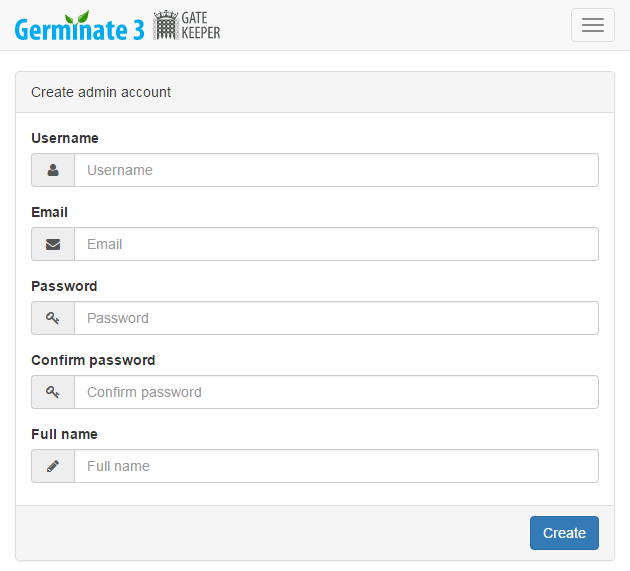
\includegraphics[scale=0.4]{img/setup/create-admin.png}
	\caption{Create admin account page}
	\label{fig:create-admin}
\end{figure}

The first time you go to the Germinate Gatekeeper website, you'll see the form shown in Figure \ref{fig:create-admin}. Fill it in to create the initial admin account. After this, you will be able to log in to Gatekeeper and create other users, database systems and set their permissions.

\subsection{Logging}
\label{subsection:logging}
Depending on your configuration (ref.\ \texttt{Germinate.Server.Logging.Enabled} in Section \ref{sec:config}), Germinate will log all server-side exceptions. This can be useful when you need to debug your version of Germinate.

The log files are stored to this location: \texttt{<Tomcat Directory>/temp/logs/}. Each instance of Germinate uses its own log files to avoid mix-ups.

\subsection{Docker}
Since version 3.3.1, a Germinate Demo Application is available as a Docker image. Please consult our website for more details:
\begin{center}
	\url{https://ics.hutton.ac.uk/germinate/germinate-docker-image}
\end{center}
\section{Configuration}
\label{sec:config}
This section will highlight some of the configurations of {\germinate}. The configurations are stored in the file \texttt{\instanceStuff/<project.name>/config.properties}. Currently the following settings are available:

\begin{lstlisting}[style=Properties]
Germinate.Database.Username=<username for the database>
Germinate.Database.Password=<password for the database

Germinate.Database.Server=<server of the germinate database>
Germinate.Database.Name=<name of the germinate database>
Germinate.Database.Port=<port for database connection>

Gatekeeper.URL=<base url of gatekeeper>
Gatekeeper.Database.Server=<server of the gatekeeper database>
Gatekeeper.Database.Name=<name of the gatekeeper database>
Gatekeeper.Database.Port=<port for database connection>

Gatekeeper.BCrypt.Rounds=<number of rounds for the bcrypt hashing algorithm>
Gatekeeper.Registration.Enabled=<allow user registration?>
Gatekeeper.Registration.Needs.Approval=<user registration needs manual approval?>

Germinate.UseAuthentication=<users have to log in to see data?>
Germinate.CookieLifespanMinutes=<the lifespan of cookies in minutes>
Germinate.Debug=<enable to see sql queries run on the server>
Germinate.KeepTemporaryFileForHours=<how long should temporary files be kept?>
Germinate.UploadSizeLimitMB=<file size limit of uploads in MB>
Germinate.AvailablePages=<list of comma separated pages that are available for this instance of germinate>

Germinate.ShowHomeOnLogin=<show the content of the home page on the login page as well?>

Germinate.Server.Logging.Enabled=<should exceptions be logged on the server?>

Germinate.IsUnderMaintenance=<is the server under maintenance?>

Germinate.IsReadOnly=<is the database in read-only mode?>

Germinate.ExternalDataFolder=<optional external data directory outside tomcat>

Germinate.HideIdColumns=<should internal id columns be hidden from tables?>

Germinate.Gallery.Images.Per.Page=<determines the number of images per page>

GoogleAnalytics.Enabled=<should google analytics be enabled?>
GoogleAnalytics.TrackingId=<the google analytics tracking id>

CookieNotifier.Enabled=<should the cookie notifier for EU cookie law be enabled?>

Germinate.Template.CustomMenu=<the custom menu structure in XML format>

Germinate.Template.CategoricalColors=<colors used for some of the charts>
Germinate.Template.GradientColors=<colors used for the gradients>
Germinate.Template.Social.ShowFacebook=<show facebook share button?>
Germinate.Template.Social.ShowTwitter=<show twitter share button?>
Germinate.Template.Social.ShowGooglePlus=<show google+ share button?>
Germinate.Template.Logo.Contains.Link=<does the svg logo contain links?>
Germinate.Template.Show.Parallax.Banner=<show parallax image banner?>

Germinate.Template.EmailAddress=<contact email email address>

Germinate.Template.Title=<title of the germinate instance>
Germinate.Template.DatabaseName=<name of the germinate instance>
Germinate.Template.TwitterLink=<twitter link>

Path.Java=<path to the java installation>
Path.R=<path to the r installation>
\end{lstlisting}
\noindent
All items starting with \texttt{Germinate.Database} have already been discussed in Section \ref{sec:germinate-config}. Items starting with \texttt{Gatekeeper.Database} can be configured analogously.

We will now explain the meaning and possible settings of all the items. Non-optional properties are marked with "$\circ$" whereas "$*$" marks properties that are non-optional if you want to use the associated functionality. Unmarked properties either have a default value shown in \textbf{bold} or aren't crucial for {\germinate} to work properly.

\label{sec:config-properties}
\begin{description}
	\item[\texttt{Germinate.Database.Username}\nonoptional] \floatright{[String]}\\The MySQL username used for the {\germinate} database.
	\item[\texttt{Germinate.Database.Password}\nonoptional] \floatright{[String]}\\The MySQL password associated with the username.
	\item[\texttt{Germinate.Database.Server}\nonoptional] \floatright{[String]}\\The server MySQL is running on.
	\item[\texttt{Germinate.Database.Name}\nonoptional] \floatright{[String]}\\The name of the {\germinate} database.
	\item[\texttt{Germinate.Database.Port}\nonoptionalif] \floatright{[$x\in\{0,\dots,49151\}$]}\\The port number to use for the database connection.
	\item[\texttt{Gatekeeper.URL}\nonoptionalif] \floatright{[URL]}\\The URL of {\gatekeeper}. This is required if the registration feature is enabled. Refer to property \texttt{Germinate.Registration.Enabled} and Section \ref{sec:registration}.
	\item[\texttt{Gatekeeper.Database.Server}\nonoptionalif] \floatright{[String]}\\The server MySQL is running on.
	\item[\texttt{Gatekeeper.Database.Name}\nonoptionalif] \floatright{[String]}\\The name of the {\gatekeeper} database.
	\item[\texttt{Gatekeeper.Database.Port}\nonoptionalif] \floatright{[$x\in\{0,\dots,49151\}$]}\\The port number to use for the database connection.
    \item[\texttt{Gatekeeper.BCrypt.Rounds}] \floatright{[$x\in \{4, \dots, \textbf{10}, \dots, 31\}$]}{\gatekeeper} uses BCrypt to hash passwords. The number of rounds determines how long the hashing will take. A larger number will make it harder to use brute-force to find the password, but at the same time it will influence how long users will have to wait for their password to be verified. The default is a value of $10$ which results in $2^{10}$ rounds. Increasing this to $11$ will \textbf{double the runtime} to $2^{11}$.
    \item[\texttt{Gatekeeper.Registration.Enabled}] \floatright{[true \pipe \textbf{false}]}{\germinate} and Gatekeeper support user registration. If this property is set to \texttt{true}, users will be able to register for access to your instance of Germinate. The registration will be accessible from the login page. See Section \ref{sec:registration} for more details.
    \item[\texttt{Gatekeeper.Registration.Needs.Approval}] \floatright{[\textbf{true} \pipe false]}\\If registration is enabled, there are two ways how users are approved for access to {\germinate}. If this property is set to \texttt{false}, users will automatically be approved and can start using {\germinate} right away. If this is not what you want, set this to \texttt{false} which will require you to approve requests manually through the Gatekeeper interface. Users will be notified with your decision via mail.
    \item[\texttt{Germinate.UseAuthentication}] \floatright{[true \pipe \textbf{false}]}\\If set to \texttt{true}, the user will have to log in using the credentials stored in {\gatekeeper}, otherwise no login procedure is required.
    \item[\texttt{Germinate.CookieLifespanMinutes}] \floatright{[$x\in\mathbb N^+$; default: \textbf{1440}]}\\The lifespan of all cookies given in minutes.
    \item[\texttt{Germinate.Debug}] \floatright{[true \pipe \textbf{false}]}\\Set to \texttt{true} if you want to see the SQL queries that are run against the database on each page. This is very handy when debugging or searching for errors. However, this should \textbf{never} \label{key}be used in production use, since it exposes the database internals.
    \item[\texttt{Germinate.KeepTemporaryFileForHours}] \floatright{[$x\in\mathbb N^+$; default: \textbf{24}]}\\The amount of hours temporary files should be kept for. Temporary files are generated whenever the user wants to download parts of the database. They are kept locally at least for the given amount of hours and after this amount of time they will be deleted the next time a user requests any temporary file.
    \item[\texttt{Germinate.UploadSizeLimitMB}] \floatright{[Float; default \textbf{0.5}]}\\The file size limit of uploads in MB.
    \item[\texttt{GoogleAnalytics.Enabled}] \floatright{[true \pipe \textbf{false}]}{\germinate} supports Google Analytics. Page navigation as well as user interactions will be tracked if this property is set to \texttt{true}.
    \item[\texttt{GoogleAnalytics.TrackingId}\nonoptionalif] \floatright{[String]}\\ The tracking id provided by Google Analytics.
    \item[\texttt{CookieNotifier.Enabled}] \floatright{[true \pipe \textbf{false}]}\\ In accordance with the EU Cookie Law \cite{CookieLaw} we provide a notify banner at the bottom of the page that informs users that we use cookies. Set this to \texttt{false} to disable this banner.
    \item[\texttt{Germinate.AvailablePages}\nonoptional] \floatright{[CSV]}\\Not all pages are useful for all instances of {\germinate}. List the names of those pages that should be available for this instance in a comma-separated fashion, \eg \texttt{climate, megaEnvironments, gallery}.
    \item[\texttt{Germinate.ShowHomeOnLogin}] \floatright{[true \pipe \textbf{false}]}\\If set to \texttt{true}, the login page will show the content of the home page as well. If set to \texttt{false}, the login page will only contain the text fields for the username and password.
    \item[\texttt{Germinate.Server.Logging.Enabled}] \floatright{[true \pipe \textbf{false}]}\\If set to \texttt{true}, exceptions will be logged on the server side. Otherwise, they will only be forwarded to the client and the client decides what to do with them.
    \item[\texttt{Germinate.IsUnderMaintenance}] \floatright{[true \pipe \textbf{false}]}\\If set to \texttt{true}, the web interface will be completely disabled, just showing a notification that the system is under maintenance.
    \item[\texttt{Germinate.IsReadOnly}] \floatright{[true \pipe \textbf{false}]}\\If set to \texttt{true}, the web interface will not allow the user to perform changes to the database, i.e., the generation/modification of user-created content will be disabled.
    \item[\texttt{Germinate.ExternalDataFolder}\nonoptionalif] \floatright{[Path]}\\If this property is set, {\germinate} will use the given path to look for files like images, data files and external applications. If the property is not set, {\germinate} will use the internal folders. This option can be useful if your data is huge and you don't want to include it in the generated war file, but rather want to store it in a different location on the server. Make sure that {\germinate} has read and write access to this folder.
    \item[\texttt{Germinate.HideIdColumns}] \floatright{[true \pipe \textbf{false}]}\\
    If set to \texttt{true}, the internal id column will be hidden from all tables.
    \item[\texttt{Germinate.Gallery.Images.Per.Page}] \floatright{[$x\in\mathbb N^+$; default: 16]}\\This setting determines how many images are shown per page on the gallery page.
    \item[\texttt{Germinate.Gallery.Make.Thumbnails.Square}] \floatright{[true \pipe \textbf{false}]}\\If set to \texttt{true}, the automatically generated thumbnails of images will be square to keep a uniform look across all thumbnails. The default is \texttt{false} to keep it consistent with previous versions.
    \item[\texttt{Germinate.Template.CustomMenu}\nonoptionalif] \floatright{[XML]}\\This allows you to customize the main menu of {\germinate}. Please consult Section \ref{sec:menu} for more details and an example.
    \item[\texttt{Germinate.Template.CategoricalColors}\nonoptional] \floatright{[CSV(HEX)]}\\A list of comma separated HEX color values (including the hash) that are used to color categories in some of the charts.
    \item[\texttt{Germinate.Template.GradientColors}] \floatright{\parbox[t][][t]{9cm}{[CSV(HEX); default: \textbf{\texttt{\#000000}}, \textbf{\texttt{\#570000}}, \textbf{\texttt{\#ff0000}}, \textbf{\texttt{\#ffc800}}, \textbf{\texttt{\#ffff00}}, \textbf{\texttt{\#ffffff}}]}}\\A list of comma separated HEX color values (including the hash) that are used for gradients (low to high).
    \item[\texttt{Germinate.Template.Social.ShowFacebook}] \floatright{[true \pipe \textbf{false}]}\\Set to true if a Facebook share button should appear on the site.
    \item[\texttt{Germinate.Template.Social.ShowTwitter}] \floatright{[true \pipe \textbf{false}]}\\Set to true if a Twitter share button should appear on the site.
    \item[\texttt{Germinate.Template.Social.ShowGooglePlus}] \floatright{[true \pipe \textbf{false}]}\\Set to true if a Google\texttt{+} share button should appear on the site.
    \item[\texttt{Germinate.Template.UseToggleSwitches}] \floatright{[\textbf{true} \pipe false]}\\Set to true if you want to use toggle switches instead of two radio buttons whenever the user has to decide between a "yes" and a "no" option.
    \item[\texttt{Germinate.Template.Logo.Contains.Link}] \floatright{[true \pipe \textbf{false}]}\\Set to true if the main website logo SVG file contains links. In that case, {\germinate} will disable the default logo link to "home" and prioritize the SVG-internal links.
    \item[\texttt{Germinate.Template.Show.Parallax.Banner}] \floatright{[\textbf{true} \pipe false]}\\Determines if the parallax scrolling image banner is shown at the top of selected pages or not.
    \item[\texttt{Germinate.Template.EmailAddress}] \floatright{[E-Mail]}\\The email address that will be displayed on the page as a contact address.    
    \item[\texttt{Germinate.Template.Title}] \floatright{[String]}\\The text to show in the browser title.
    \item[\texttt{Germinate.Template.DatabaseName}] \floatright{[String]}\\The text to show in the "featured banner" on the page.
    \item[\texttt{Germinate.Template.TwitterLink}] \floatright{[URL]}\\The link to the associated Twitter account.
    \item[\texttt{Path.Java}] \floatright{[String]}\\The path to the Java installation. This is optional, since {\germinate} can get it from the JVM it's running in. However, if required, {\germinate} can be pointed to a different Java version and will use this to run all internal Java calls.
    \item[\texttt{Path.R}\nonoptionalif] \floatright{[String]}\\The path to the R installation.
\end{description}
\noindent
Any change to these properties will automatically be picked up by {\germinate}, i.e. no reload of the web interface on Tomcat is required.

There is also a configuration page directly in {\germinate}. This page is only visible to administrators and can be reached by going to:
\begin{center}
	\texttt{http://<Your web server>:8080/<project.name>/\#admin-config}
\end{center}
\noindent An example of this page can be seen in Figure \ref{fig:admin-config}.

\begin{figure}
	\centering
	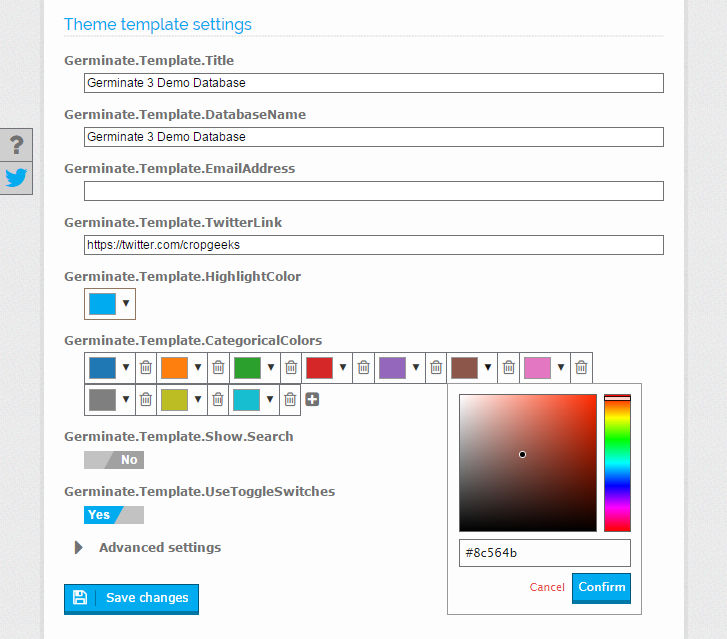
\includegraphics[width=1\textwidth]{img/configuration/admin-config.png}
	\caption{The {\germinate} configuration page available to administrators.}
	\label{fig:admin-config}
\end{figure}

\subsection{{\germinate} Menu}
\label{sec:menu}
{\germinate} uses a predefined menu structure by default. This default menu setup is based on what we think is a reasonable structure. However, even we are not infallible, so we decided to make the menu customizable.

We will now explain how you can define your own, custom menu structure and we will then give an example of how this can be used.

\subsubsection{Structure}
The menu of {\germinate} can be defined in XML format. We will explain this format using the example below:

\begin{lstlisting}[style=Xml]
<menu>
	<item key="home" icon="mdi-home-circle">
		<label key="en_GB">Home</label>
		<label key="de_DE">Home</label>
	</item>
	<item key="category.data">
		<label key="en_GB">Data</label>
		<label key="de_DE">Daten</label>
		<item key="browse-accessions">
			<label key="en_GB">Accessions</label>
			<label key="de_DE">Muster</label>
		</item>
		<item key="category.molecular">
			<label key="en_GB">Molecular data</label>
			<label key="de_DE">Molekulare Daten</label>
			<item key="genotype-datasets">
				<label key="en_GB">Genotypes</label>
				<label key="de_DE">Genotypen</label>
			</item>
			<item key="map-details">
				<label key="en_GB">Maps</label>
				<label key="de_DE">Molekulare Karten</label>
			</item>
		</item>
	</item>
	<item key="category.environment">
		<label key="en_GB">Environment</label>
		<label key="de_DE">Umwelt</label>
		<item key="geographic-search">
			<label key="en_GB">Geographic search</label>
			<label key="de_DE">Geografische Suche</label>
		</item>
	</item>
</menu>
\end{lstlisting}
\noindent
This will result in the following menu structure:\\
\\
\begin{tabular}[t]{@{}>{\raggedright\arraybackslash}p{0.5\textwidth}}
	\textbf{British English}:
	\begin{itemize}
		\item Home
		\item Data
		\begin{itemize}
			\item Accessions
			\item Molecular data
			\begin{itemize}
				\item Genotypes
				\item Maps
			\end{itemize}
		\end{itemize}
		\item Environment
		\begin{itemize}
			\item Geographic search	
		\end{itemize}
	\end{itemize}
\end{tabular}
\begin{tabular}[t]{@{}>{\raggedright\arraybackslash}p{0.5\textwidth}}
	\textbf{German}:
	\begin{itemize}
		\item Home
		\item Daten
		\begin{itemize}
			\item Muster
			\item Molekulare Daten
			\begin{itemize}
				\item Genotypen
				\item Genetische Karten
			\end{itemize}
		\end{itemize}
		\item Umwelt
		\begin{itemize}
			\item Geographische Suche
		\end{itemize}
	\end{itemize}
\end{tabular}
\noindent
We will now explain the individual elements of the XML file:
\begin{description}
	\item[\texttt{menu}] The root element of the XML file.
	\item[\texttt{item}] This is used for any menu element. This can either be a link to an actual page, or a submenu.
	\item[\texttt{item key}] If this item represents an actual {\germinate} Page (cf. Section \ref{sec:pages}) then this has to be the name of the page. If this item is a sub-menu, then this has to be a unique id.
	\item[\texttt{item icon}] The icon that should be used for this menu item. It has to be one of the icons from \url{https://materialdesignicons.com/}. They are all prefixed with "\texttt{mdi-}". If no icon is provided, no icon will be shown.
	\item[\texttt{label}] Labels are used as the text content of the menu item, i.e. what the user will see. Every item has to provide this information for ALL of the supported languages (cf. Section \ref{sec:i18n}).
	\item[\texttt{label key}] The locale of the supported language.
\end{description}
\section{Features}
In this section, we will highlight the main features of Germinate. This section will expand as we add new features.

\subsection{Internationalization and Localization}
\label{sec:features_i18n}
Germinate fully supports internationalization for an unlimited number of languages. Every text that you can see on the web interface can be localized. The language used on start-up is chosen based on the browser settings, but the user can easily switch to a different language by selecting it from the combo box at the bottom of the page. Have a look at Section \ref{sec:example_i18n} for usage details.

\subsection{Help}
Every page can include a help text. This text will be shown when the user clicks on the help icon. The main purpose of this help is to explain features of the current page to the user. As a result, the page itself does not look cluttered, but the user is still able to find help if the workflow of the page is not obvious.

\subsubsection{Tours}
In addition to a simple help text, we also offer the ability to add interactive tours to the pages. An interactive tour can be described as a sequence of help texts with visual feedback on the page itself. These steps can guide the user through the page and explain every step in detail. An example of a tour step can be seen in Figure \ref{fig:tour}.

\begin{figure}
    \centering
    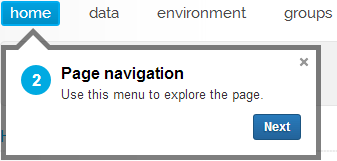
\includegraphics[scale=0.7]{img/features/tour-example2.png}
    \caption{Example step of a tour}
    \label{fig:tour}
\end{figure}

\subsection{News}
The Germinate web interface contains a place holder to show the latest news of the project. On the database side, these news are stored in two tables and can be updated at any time. The web interface will check the availability of news and show the three latest entries at the bottom of the page. Changes on the database side will immediately be visible on the website.

\subsection{Notifications}
Germinate offers a set of essential notification types. The notification system is based on Toastr \cite{Toastr}. All notifications fully support internationalization as well as custom styling. The currently available notification types can be seen in Figure \ref{fig:notification-types}. Section \ref{sec:example_notification} contains an example showing how to use the notification system.

\begin{figure}
    \centering
    \begin{subfigure}[t]{0.3\textwidth}
        
\includegraphics[width=\textwidth]{img/features/notification_success.png}
        \caption{Success}
    \end{subfigure}
    \hspace*{0.1\textwidth}
    \begin{subfigure}[t]{0.3\textwidth}
        
\includegraphics[width=\textwidth]{img/features/notification_error.png}
        \caption{Error}
    \end{subfigure}\\
    \begin{subfigure}[t]{0.3\textwidth}
        
\includegraphics[width=\textwidth]{img/features/notification_warning.png}
        \caption{Warning}
    \end{subfigure}
    \hspace*{0.1\textwidth}
    \begin{subfigure}[t]{0.3\textwidth}
        
\includegraphics[width=\textwidth]{img/features/notification_info.png}
        \caption{Info}
    \end{subfigure}
    \caption{Available notifications}
    \label{fig:notification-types}
\end{figure}

\subsection{Available pages}
\label{sec:pages}
This section gives an overview of all the pages that are available for Germinate. Based on your requirements and the data that is available, you can decide which pages should actually be available on the web interface and hide all others. The set of available pages can be changed dynamically without having to re-deploy the application. This gives you the freedom to customize your Germinate experience just as you please.

A table with the available pages can be found in Table \ref{tab:pages}.

\begin{longtable}{p{\dimexpr 0.27\linewidth-2\tabcolsep}p{\dimexpr 0.45\linewidth-2\tabcolsep}p{\dimexpr 0.28\linewidth-2\tabcolsep}}
	%\caption{List of all available pages in Germinate 3}\\
	\toprule
	\textbf{Page name}     & \textbf{Description} & \textbf{Required data} \\
	\midrule\midrule
	\endhead
	about-germinate        & Shows information about Germinate & - \\ \midrule
	about-project          & Shows information about the project & - \\ \midrule
	accessions-for-collsite & Shows available accessions for the selected collecting site & \cellwrap{germinatebase,\\locations,\\locationtypes,\\countries}\\ \midrule
	acknowledgements       & Shows acknowledgements & - \\ \midrule
	allele-freq-dataset & Shows the datasets containing allele frequency data & \cellwrap{datasets,\\datasetstates,\\datasetpermissions,\\experiments} \\ \midrule
	allele-freq-export  & Page showing the settings used for the export of allele frequency data & \cellwrap{allelefrequencydata,\\datasets,\\datasetstates,\\datasetpermissions,\\germinatebase,\\groups,\\groupdatasets\\grouptypes,\\maps} \\ \midrule
	allele-freq-result  & Page showing the result of the allele frequency data export & \cellwrap{allelefrequencydata,\\datasets,\\datasetstates,\\datasetpermissions,\\groups,\\maps} \\ \midrule
	browse-accessions       & A paginated table containing all the accessions in the database. & \cellwrap{countries,\\germinatebase,\\locations,\\taxonomies,\\subtaxa} \\ \midrule
	cart                   & The cart contains marked accessions. & \cellwrap{germinatebase} \\ \midrule
	categorical-datasets    & Shows the datasets containing categorical data & \cellwrap{datasets,\\datasetstates,\\datasetpermissions,\\experiments} \\ \midrule
	categorical-export      & Page showing the settings used for the export of categorical data & \cellwrap{datasets,\\datasetstates,\\datasetpermissions,\\germinatebase,\\groups,\\groupdatasets,\\grouptypes\\phenotypes} \\ \midrule
	climate                & Page showing the settings used for the export of categorical data & \cellwrap{climatedata,\\climates,\\groups,\\units,\\groups,\\grouptypes,\\phenotypes} \\ \midrule
	collsite-treemap        & Page showing a treemap of the collectingsites & \cellwrap{countries,\\germinatebase,\\locations} \\ \midrule
	cookie                 & Page showing the cookie policy & - \\ \midrule
	dataset-overview       & Page showing all the available datasets & \cellwrap{datasets,\\datasetstates,\\datasetpermissions,\\experiments,\\experimenttypes} \\ \midrule
	experiment-details     & Page showing all datasets that are part of an experiment & \cellwrap{datasets,\\datasetstates,\\datasetpermissions,\\experiments,\\experimenttypes} \\ \midrule
	gallery                & A gallery of images & \cellwrap{images,\\imagetypes} \\ \midrule
	genotype-datasets       & Shows the datasets containing genotypic data & \cellwrap{datasets,\\datasetstates,\\datasetpermissions,\\experiments} \\ \midrule
	genotype-export         & Page showing the settings used for the export of genotypic data & \cellwrap{datasets,\\datasetstates,\\datasetpermissions,\\genotypes,\\germinatebase,\\groups,\\groupdatasets\\grouptypes,\\mapdefinitions,\\maps,\\markers} \\ \midrule
	geographic-search       & Page used to query for collecting sites by distance to a query location & \cellwrap{countries,\\locations} \\ \midrule
	geography              & Page that shows different visualizations of collecting sites on maps & \cellwrap{countries,\\locations} \\ \midrule
	groups				   & Page listing defined groups of accessions, markers, ... & \cellwrap{groupmembers,\\groups,\\grouptypes} \\ \midrule
	help				   & Page with general help information & - \\ \midrule
	home				   & Welcome page of the web interface & - \\ \midrule
	login                  & The login page of Germinate & - \\ \midrule
	logout				   & The logout page of Germinate & - \\ \midrule
	map-details			   & Page listing the details about a selected map & \cellwrap{mapdefinitions,\\mapfeaturetypes,\\maps,\\markers} \\ \midrule
	marker-details          & Page listing the details about a selected marker & \cellwrap{datasets,\\genotypes,\\markers} \\ \midrule
	mega-environments       & Page with the mega environments & \cellwrap{countries,\\germinatebase,\\locations,\\megaenvironmentsdata,\\megaenvironments,\\megaenvironmentsource,\\soils}\\ \midrule
	news				   & List of the latest news & \cellwrap{news,\\newstypes} \\ \midrule
	passport			   & Page listing the details about a selected accession & \cellwrap{countries,\\germinatebase,\\locations,\\subtaxa,\\taxonomies} \\ \midrule
	search				   & Shows search results & \cellwrap{countries,\\germinatebase,\\locations,\\markers,\\mapdefinitions,\\mapfeaturetypes} \\ \midrule
	trials                 & Page with different visualizations of trials data & \cellwrap{germinatebase,\\phenotypes,\\trialsdata} \\ \midrule
	trials-datasets         & Shows the datasets containing trials data & \cellwrap{datasets,\\datasetstates,\\datasetpermissions,\\experiments} \\ \midrule
	trials-individual       & Shows visualizations of trials data for an accession and a phenotype & \cellwrap{trialsdata,\\trialseries,\\trialsites} \\ \midrule
	\bottomrule
	\label{tab:pages}
\end{longtable}

\subsubsection{User registration}
\label{sec:registration}

Germinate can be used with and without authentication. This means that you can decide if you want to restrict access to your Germinate instance to registered users. If you decide to do so, you'll need people to be able to register. The registration form of Germinate (Figure \ref{fig:user_registration_registration}) provides a concise and easy way to register. If you choose to use a disclaimer that potential new users have to accept, this will appear before the form is visible. Once the user completes the form, they will either get access right away or you need to approve the new users manually. This is based on the setting of the property \texttt{Gatekeeper.Registration.Needs.Approval} (see Section \ref{sec:config-properties} for help). If you choose to use the approval approach, you'll see the screen shown in Figure \ref{fig:user_registration_approval} after selecting "Approve users" in Gatekeeper. The user will be notified with your decision.

\begin{figure}
    \centering
    \begin{subfigure}[b]{0.475\textwidth}
        \centering
        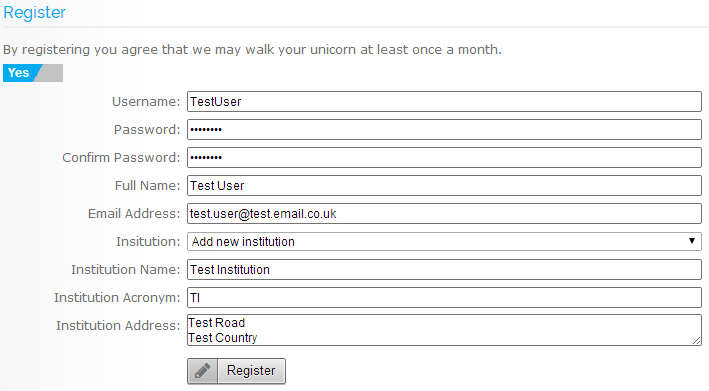
\includegraphics[width=1.0\textwidth]{img/features/registration.png}
        \caption{Registration form on the Germinate 3 site}
        \label{fig:user_registration_registration}
    \end{subfigure}
    \hspace*{0.5cm}
    \begin{subfigure}[b]{0.475\textwidth}
        \centering
        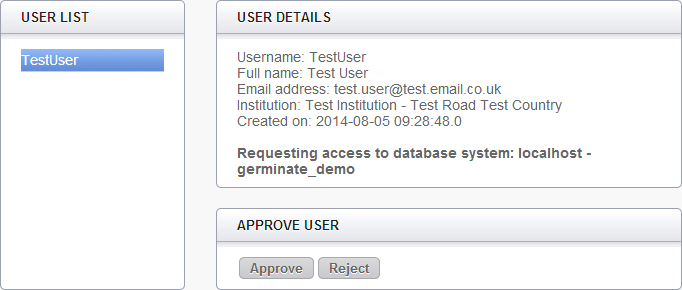
\includegraphics[width=1.0\textwidth]{img/features/registration-approve.png}
        \caption{Approval page on the Gatekeeper page}
        \label{fig:user_registration_approval}
    \end{subfigure}
    \caption{User registration}
    \label{fig:user_registration}
\end{figure}

\subsubsection{Groups}
Germinate allows you to define groupings of various items which makes exporting or visualizing data more comfortable. An intuitive example of groups are accession groups. A group of accessions can contain accessions that are similar to each other or a list of accessions that you want to export against a map for visualization in Flapjack.

A new group can be created with a couple of clicks: First, select the type of group that you want to create, \eg accession group, collecting site group, marker group etc. Afterwards, create a new group by just entering the name of the new group.

To delete group members, just select the group that you want to modify and check the items to remove in the table. Afterwards click on the delete button below the table. To delete a complete group, click on the delete icon next to the group selection box.

\paragraph{Searching by item criteria}
Searching for the items you want to add to the group is very straight forward. Germinate supports searching on almost all columns of the table containing the data. Examples are: "country of origin", "region", "state, "latitude", "longitude" and "elevation" for collecting sites. You can restrict your search by specifying multiple criteria. The criteria currently have the following structure:
\begin{center}
    <column> \{less than, greater than, equal\} <value>
\end{center}
\noindent
Multiple criteria can be combined using logical conjunction ($\land$, AND) and disjunction ($\lor$, OR). Note that conjunction binds stronger than disjunction making the order of criteria important. An example can be seen in Figure \ref{fig:group_search} (\subref{fig:group_search_item}). The example requests all accessions with "mexico" as their country of origin \textbf{or} those accessions with a name starting with "A".

\paragraph{Searching by climate criteria}
If climate data is available, Germinate allows to select subsets of items based on a combination of climate criteria. The process is identical to the one seen above. Figure \ref{fig:group_search} (\subref{fig:group_search_climate}) shows an example. The example requests collecting sites having a maximal average temperature of less than 30 \textbf{and} having a minimal average temperature of more than 20.

\begin{figure}
    \centering
    \begin{subfigure}[t]{1.0\textwidth}
        \centering
        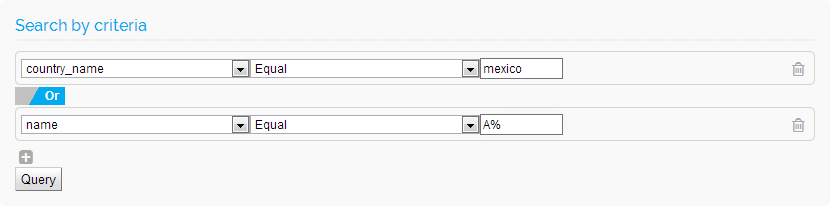
\includegraphics[scale=0.5]{img/features/groups_item.png}
        \caption{Accession search by item criteria}
        \label{fig:group_search_item}
    \end{subfigure}
    \\
    \begin{subfigure}[t]{1.0\textwidth}
        \centering
        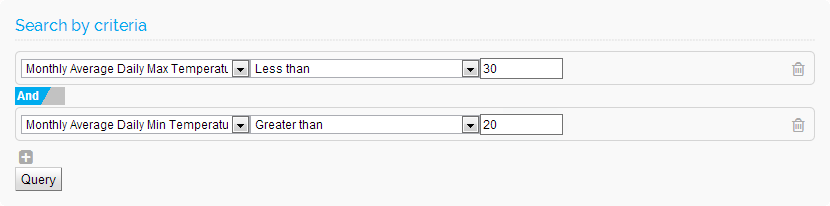
\includegraphics[scale=0.5]{img/features/groups_climate.png}
        \caption{Collecting site search by climate criteria}
        \label{fig:group_search_climate}
    \end{subfigure}
    \caption{Examples of group searches}
    \label{fig:group_search}
\end{figure}

\subsubsection{Data}
The main purpose of Germinate is to store multiple data types, let the user query them and create visualizations of the data. In this section, we will give an overview of the different data types and visualizations Germinate supports.

\paragraph{Browse accessions and Passport}
This page lists all accessions stored in Germinate in a tabular format. The table is sortable and supports pagination, \ie it will split into multiple pages if necessary to ensure readability. Clicking on an accession will take you to the passport page. The passport page contains all the meta information that is available for the selected accession such as name, genus, breeder information, images and annotations.

Passport data tends to be quite fragmented so its perfectly possible that we have limited data for some lines while others have a full complement.

\paragraph{Maps and Markers}
The map page shows a list of available maps defined in Germinate. Clicking on a map will show its member markers with detailed information about chromosome and position on the chromosome. In turn clicking on a marker shows information about the molecular and genotype information about this marker as well as a list of the datasets the marker is contained in. Click on the dataset to reveal the genotypes for the selected combination of marker and dataset.

\paragraph{Genotype data export}
The genotype information held in Germinate can be exported as tab separated values as well as in a format that is compatible with the genotype data viewer \textit{Flapjack}. The process of exporting the data is structured like a wizard dialog.

First you need to select the dataset containing the data that you want to export. The second wizard page shows the accession and marker groups as well as the maps that are visible to you. Just select the items that you want to export. The \textit{Crap Data Filter} (CDF) can be enabled to prune markers from the export that exceed a certain threshold for missing or heterozygous values.
Finally, you need to select the file containing the raw data. The third page finally contains your exported data in both already mentioned formats. If the CDF was enabled, this page will show the list of deleted markers for your convenience.\\
\\
\textbf{Note}: Make sure that all the files that contain your genotype data are encoded with UTF-8.

\paragraph{Allele frequency data export}
Exporting allele frequency data is almost identical to the genotype data export. The first two wizard pages are again used to select datasets and accession and marker groups. The third page differs from the genotype export, because this is the page where you actually can decide how you want your data to be binned. The binning step is necessary for visualization in Flapjack. Currently, there are three types of binning mechanisms: \textit{Equal-width binning}, \textit{Split point binning} and \textit{automatic binning}.

Equal-width binning will result in a specified number of bins all having the same width. Split point binning is an extension of this principle. It lets you specify a split point and a number of bins to either side of the split point. The parts to the left and the right of the split point are binned according to the equal-width binning principle. Automatic binning is more sophisticated. It will automatically determine the best splitting points given a number of bins. The resulting binning will contain approximately the same number of items in each bin. Another name for this principle is consequently equal-size binning.

\paragraph{Phenotype data export}
The phenotype export process is structured similarly to the genotype export. In the first step you can select the dataset containing your data. The next page will show the available phenotypes and accession groups that can be selected for export.

Now you can select if you just want to have a look at the data or if you want to be able to download it as well. Check the checkbox at the bottom of the page to create a downloadable file containing the data. Pressing continue will start the export process. Once the date is returned from the server, it will be displayed at the bottom of the page. A download link will be attached below the table if you decided to select data download in the previous step.

\subsubsection{Environment}
Environmental data can include climate data, GIS (Geographic information system) data, soil data and many more. Germinate can store all that information and use it to create meaningful visualizations and overviews.

\paragraph{Geography}
The geography page visualizes the geographic data contained in Germinate on Google Maps. So far the only instance that holds geographic information are the collecting sites, for which we store latitude, longitude and altitude information.

There are three types of maps that are currently supported. The first type is a simple map with a marker for each data point in the database. This can get quite cluttered when the number of items increases. The two other types of maps pose solutions to this issue.

The first of them is a \textit{Heatmap Layer} \cite{HeatmapLayer} for the map. A heatmap is a data visualization technique where the data points are not represented individually, but instead they are used to calculate a density function which is then plotted on top of the Google Map. The density function assigns a high value to areas where the probability of observing data points is high and a low value to areas where this probability is low. To visualize this principle, the heatmap is color-coded.

The other alternative to individual markers is the \textit{MarkerClusterer} \cite{MarkerClusterer}. The MarkerClusterer uses a very basic grid-based clustering algorithm to group clusters located in the same area into clusters. This solution massively reduces the number of visible markers on the screens since each cluster is now represented by a marker instead of the hundreds of actual markers it contains. The clusters will be re-generated on every zoom level resulting in approximately the same number of visible clusters independent of the zoom level.

Figure \ref{fig:geography-maps} shows an example dataset containing about 1000 markers. Figure \ref{fig:geography-maps}(a) shows the individual markers and we can see that this is very cluttered. Figure \ref{fig:geography-maps}(b) and \ref{fig:geography-maps}(c) show the HeatmapLayer and MarkerClusterer respectively. 

\begin{figure}
    \begin{subfigure}[t]{0.32\textwidth}
        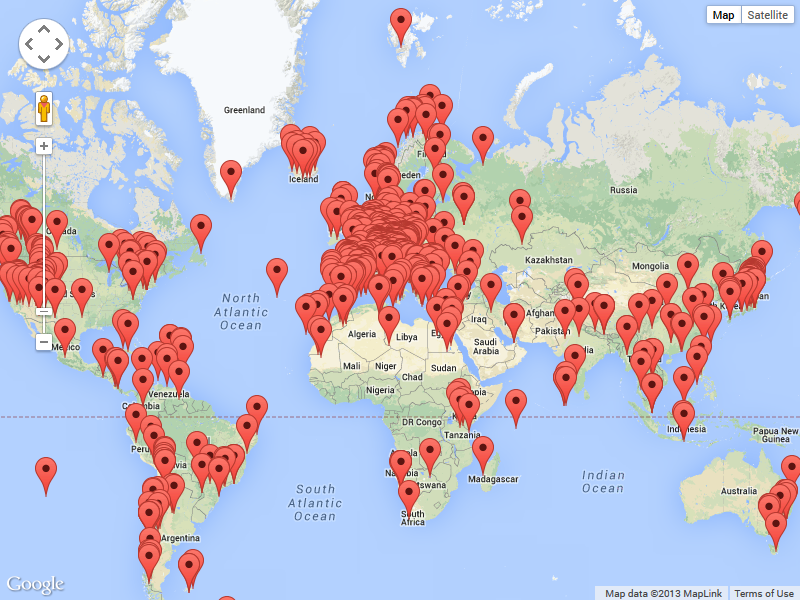
\includegraphics[width=\textwidth]{img/features/markers.png}
        \caption{Markers}
    \end{subfigure}
    ~
    \begin{subfigure}[t]{0.32\textwidth}
        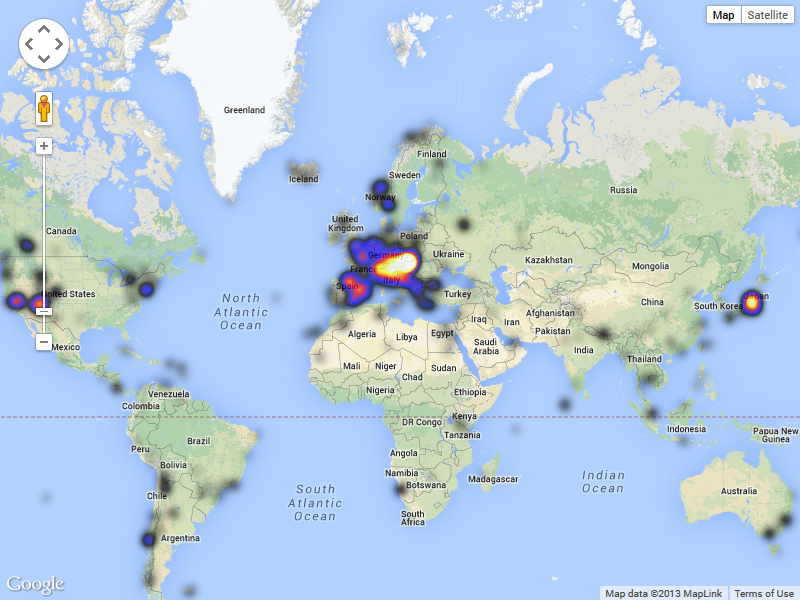
\includegraphics[width=\textwidth]{img/features/heatmap.png}
        \caption{HeatmapLayer}
    \end{subfigure}
    ~
    \begin{subfigure}[t]{0.32\textwidth}
        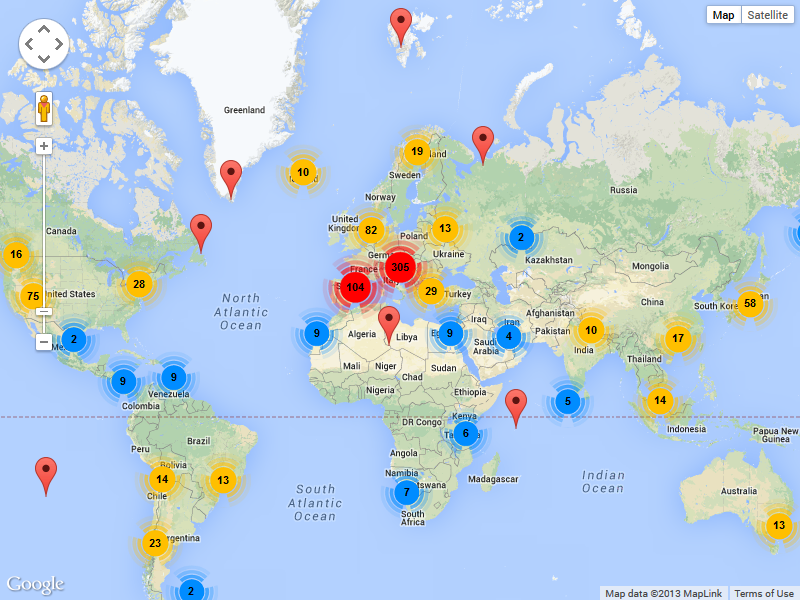
\includegraphics[width=\textwidth]{img/features/markerclusterer.png}
        \caption{MarkerClusterer}
    \end{subfigure}
    \caption{Different representations of the same geographic information}
    \label{fig:geography-maps}
\end{figure}

\paragraph{Geographic Search}
The geographic search can be used to find collecting sites with the help of a Google Map. You can either enter coordinates (latitude and longitude) directly, or scroll to the position of interest on the map. A click on the "Continue" button will list all collecting sites ordered by their distance (in km) to your query location.

\paragraph{Geographic Treemap}
Treemapping (\url{http://en.wikipedia.org/wiki/Treemapping}) is a method for displaying hierarchical data by using nested rectangles. In our case, we visualize the hierarchy of locations in a treemap. The highest level of abstraction can be defined using the \texttt{Germinate\allowbreak .CollectingsiteTreemapColumn} property described in Section \ref{sec:config-properties}. Clicking on one of the top level rectangles will zoom in and show the actual collecting sites. Clicking on those will take you to a page listing all the accessions collected at this site.

\paragraph{Mega Environments}
A mega environment can be defined as a set of areas sharing the same or very similar attributes ranging from biotic and abiotic stresses to customer preferences.

The mega environments page lists all recorded mega environments with the collecting sites located within them. Selecting a collecting site takes you to a page showing the accessions found at this site.

The data contained in both the mega environment page as well as the collecting sites page can be downloaded in KML (\textbf{K}eyhole \textbf{M}arkup \textbf{L}anguage) format allowing viewing in Google Earth \cite{GoogleEarth}.

\paragraph{Climate}
Climate data is very diverse. Everything that can be measured by sensors can be considered as climate information. Examples are precipitation, hours of daylight, temperature, frost frequency and atmospheric pressure. Germinate can store all kinds of climate data. The climate page of the Germinate web interface visualizes the contained data in a compact and understandable way. Figure \ref{fig:climate_table} shows an example visualization using color-coding of the average measured temperature for the given collecting sites.

If you have climate layer images that go along with your climate data, Germinate is able to display them on top of a Google Map below the climate chart.

\begin{figure}
    \centering
    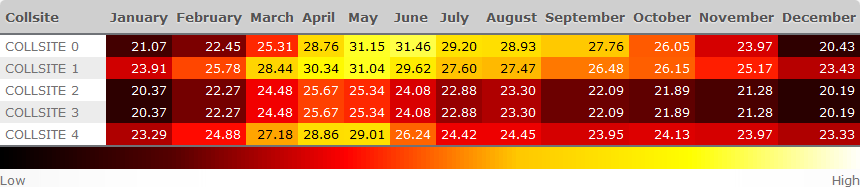
\includegraphics[scale=0.5]{img/features/climate_table.png}
    \caption{Color-coded climate table (average temperature in \textcelsius)}
    \label{fig:climate_table}
\end{figure}

\subsubsection{Image gallery}
The image gallery is an elegant way to display images that do not fit on any of the other pages. The images will be held in a table structure and can be browsed in a pagewise fashion. New images can easily be added by copying them into the following directory:
\begin{center}
    \texttt{<Apache Directory>/webapps/<project.name>/WEB-INF/classes/download}
\end{center}
There are two sub-folders called \texttt{images} and \texttt{thumbnails}. Copy the full size images into the \texttt{images} directory and small thumbnails into the \texttt{thumbnails} folder. For optimal visual appearance make sure that all the thumbnails have the same height. A height of 150px is a good reference value.

The images will be sorted by the "Last Modified Date" making sure that the newest images appear first.

\subsubsection{Search}
Every website should have a basic search feature. The search feature of Germinate allows to search for accessions, collecting sites, markers etc. by their features. You know the name of an accession? Excellent, just search for it and tell Germinate that it's the name you're searching for. Only know the ID? No problem, just use the ID instead and mark it as the ID. We use \texttt{\%} as the wildcard character. A wildcard character can be used to substitute for arbitrary other characters. As an example, \texttt{\%king\%} will match \texttt{United Kingdom}, whereas \texttt{king\%} will only match \texttt{Kingdom}. Note that we currently don't match cases during the search.

\subsection{Color Themes}
Germinate is highly customizable. We have already seen a lot of configuration options in Section \ref{sec:config-properties}. In this section we want to highlight one of the customization features in particular: color themes. The configuration properties responsible for the color theme of Germinate are:

\begin{lstlisting}[style=Properties]
Germinate.Template.HighlightColor=<main color of all highlights on the interface>
Germinate.Template.CategoricalColors=<colors used for some of the charts>
\end{lstlisting}

\noindent
We will now show how the look of Germinate can be completely changed by just setting these two properties. The default color theme of Germinate is a composition of different shades of blue (see Figure \ref{subfigure:blue-theme}). With the following property changes, we get the completely changed theme seen in Figure \ref{subfigure:red-theme}.

\begin{figure}[h]
	\centering
	\begin{subfigure}[t]{0.48\textwidth}
		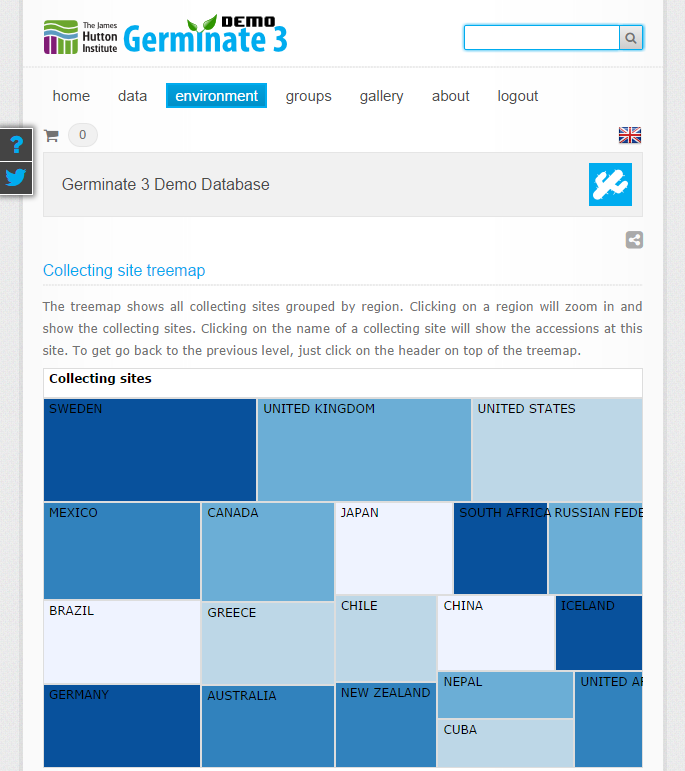
\includegraphics[width=\textwidth]{img/features/themes-blue.png}
		\caption{Default blue color theme}
		\label{subfigure:blue-theme}
	\end{subfigure}
	~
	\begin{subfigure}[t]{0.48\textwidth}
		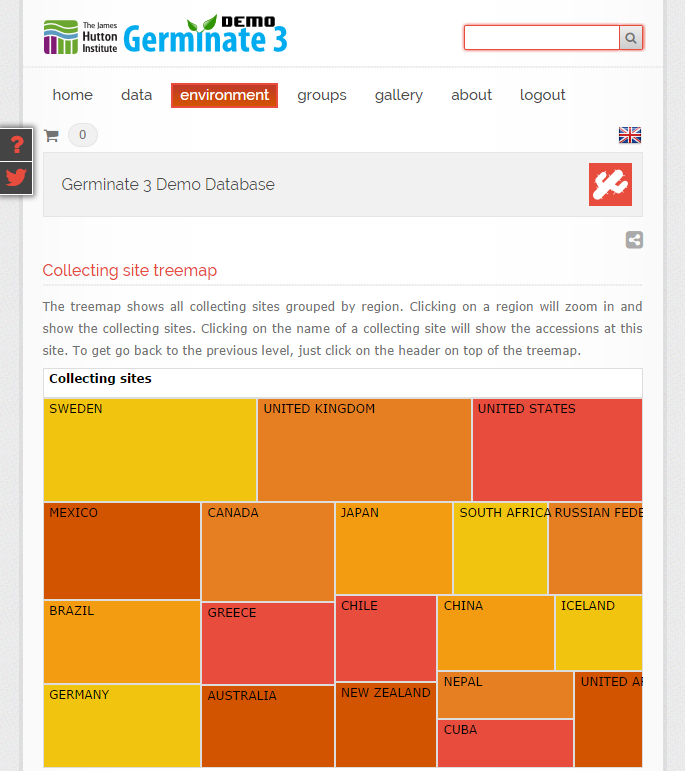
\includegraphics[width=\textwidth]{img/features/themes-red.png}
		\caption{Red color theme}
		\label{subfigure:red-theme}
	\end{subfigure}
	\caption{Different color themes}
	\label{fig:color-themes}
\end{figure}

\begin{lstlisting}[style=Properties]
Germinate.Template.HighlightColor=#e74c3c
Germinate.Template.CategoricalColors=#e74c3c,#d35400,#e67e22,#f39c12,#f1c40f
\end{lstlisting}

\noindent As you can see, the color theme affects almost all elements of the website: links, headings, backgrounds, icons, highlight effects, chart colors, etc.

Although we do our best to take care of all elements, we can't simply change the images you include, \ie the included images do not change colors based on these settings. An example is the Germinate 3 logo in both screenshots. As can be seen, it stays blue. However, all other elements that are included in the default installation of Germinate will change color according to the defined properties.

\subsection{Security}
\label{sec:example_security}
As already mentioned earlier, Germinate is equipped with a secure login system\footnote{Germinate is only as secure as the connection between client and server. Use a secure connection (TLS/SSL) to prevent password snooping.}. This feature is completely optional, but it allows you to protect your data from any unauthorized access. In this section, we will explain how the security system works and we will show what is necessary to use it properly.

\begin{figure}[h]
    \centering
    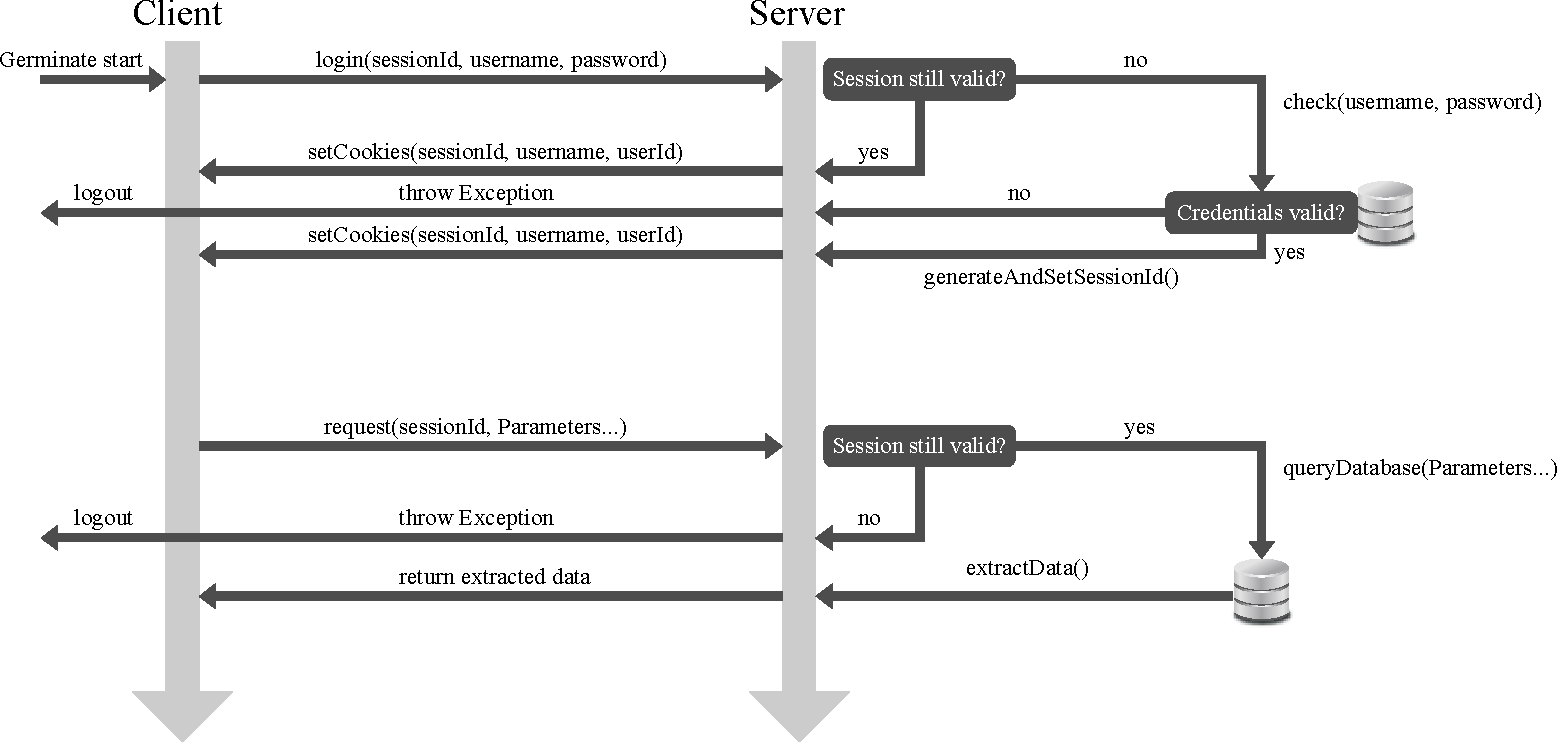
\includegraphics[scale=0.5]{img/examples/authentication.pdf}
    \caption{Authentication procedure of Germinate}
    \label{fig:authentication}
\end{figure}

Figure \ref{fig:authentication} shows the authentication process of Germinate. The figure contains two major parts. The upper part visualizes the login process, which is initialized by the user entering his/her credentials. These are sent to the server alongside any session id that is still stored in the client from previous sessions. The server will then check the session id that is received. If the id is still valid, the server will store the session id and return it to the client, which, in turn, will create a cookie containing this id.

If the session id is invalid, the server will check if the username password combination is genuine. This is done by encrypting the password and checking it against the entry in the database. If this check fails, the user will be logged out. Otherwise, the server will create a new session id, store it in the HTTP session and return it to the client, which will create a new cookie using this id. The login process is now complete and both the server (via HTTP session) and the client (via cookie) know the current session id.

For each new request that is made from the client, it will need to send the session id as the payload, \ie each remote procedure call (RPC) has to request the session id as a parameter to ensure the security of the communication. As a consequence if this, the server will receive the session id three times per request, namely via the HTTP session, via the cookie and via the payload. If all of these ids match up, the server can fulfil the client's request and return the data. However, if it fails, the user will be logged out.

As a final remark: Even if you currently do not want to enable the security feature, you should still write your code in a way that ensures it will work properly even when the security feature is enabled. Otherwise you might end up with a security leak.
\section{Structure}
\label{sec:structure}
In Section \ref{sec:structure-project}, we will explain the structure of the Germinate project. This includes the folder structure of the subversion project as well as the structure of the deployed product. Section \ref{sec:structure-database} contains information about the structure of the database itself.

\subsection{Subversion project}
\label{sec:structure-project}
\begin{figure}[h]
    \centering
    \begin{subfigure}[b]{0.49\textwidth}
        \centering
        \begin{tikzpicture}[scale=0.7, every node/.style={scale=0.7}]
			\treeroot{instance-stuff}
			\folder{your-project}{1}
			\folder{apps}{2}
			\folder{some-app}{3}
			\folder{data}{2}
			\folder{download}{2}
			\folder{images}{3}
			\folder{fullsize}{4}
			\file{accession-a.png}{5}
			\folder{thumbnails}{4}
		    \file{accession-a.png}{5}
			\folder{\dots}{3}
			\folder{download-de\textunderscore DE}{2}
			\folder{images}{3}
			\folder{fullsize}{4}
			\file{accession-a.png}{5}
			\folder{thumbnails}{4}
			\file{accession-a.png}{5}
			\folder{\dots}{3}
			\folder{modules}{2}
			\folder{core}{3}
			\file{Text.properties}{4}
			\file{Text\textunderscore de\textunderscore DE.properties}{4}
			\folder{\dots}{3}
			\folder{res}{2}
			\file{Dendrogram.R}{3}
			\folder{template}{2}
			\folder{css-images}{3}
			\folder{fonts}{3}
			\folder{images}{3}
			\file{crop.svg}{4}
			\folder{js-external}{3}
			\folder{parallax-images}{3}
			\file{parallax-about-germinate.jpg}{4}
			\file{\dots}{4}
			\file{custom.css}{3}
			\file{custom.html}{3}
			\file{favicon.ico}{3}
			\file{logo.css}{3}
			\file{logo.svg}{3}
			\file{config.properties}{2}
			\file{Germinate.gwt.xml}{2}
			\file{web.xml}{2}
			\folder{other-project}{1}
		\end{tikzpicture}
        \caption{Overall structure}
        \label{fig:project-structure-project}
    \end{subfigure}
%    \hspace*{0.1\textwidth}
    \begin{subfigure}[b]{0.49\textwidth}
        \centering
           \begin{tikzpicture}[scale=0.7, every node/.style={scale=0.7}]
			\treeroot{war}
			\folder{css}{1}
			\folder{error}{1}
			\folder{germinate}{1}
			\folder{js}{1}
			\folder{WEB-INF}{1}
			\file{germinate.jsp}{1}
			\file{germinate-css.jsp}{1}
		\end{tikzpicture}
        \caption{Web structure}
        \label{fig:project-structure-web}
    \end{subfigure}\\
    \caption{Available notifications}
    \label{fig:project-structure}
\end{figure}
\noindent
The actual subversion project of Germinate is structured as shown in Figure \ref{fig:project-structure}. Figure \ref{fig:project-structure-project} shows the overall structure of the whole project whereas Figure \ref{fig:project-structure-web} shows the structure of the files and folders related to the web side of things.

\subsubsection{Project structure}
Germinate is designed to allow custom look and feel for different projects. This means you are able to have multiple configurations of Germinate, each tailored specifically for the special needs of the individual projects. As an example we show the structure of the project "your-project" which in reality would be named after your project.

There are several sub-directories. The "apps" directory includes external applications that ship with Germinate. In this example, we include an application called "some-app". The "data" directory contains raw data files that are used during the export processes. The "download" directory contains all the data files that you want to provide as downloads on Germinate. Those can include images for the gallery, pdfs, etc. The "download-de\textunderscore DE" directory contains internationalized versions of the files found in "download". See Section \ref{sec:localized-files} for further details. The "modules" directory contains the internationalization property files for each module. In this example, there is only one module, namely the "core" module which is the basic Germinate module. Internationalized text goes here. The "res" folder can be used to host several files that are used as resources. The content of this folder is copied to the server and accessible from the server side code. In this example we have an R file that is used on the server to generate a dendrogram.

Finally, the "template" folder contains custom styling files for your individual instance of Germinate. Those include custom logos, custom css, custom html, custom JavaScript libraries, custom parallax images, fonts, a favicon, etc.

The other files in your project folder are the most important ones. They define how Germinate works. We'll give a detailed description of each file below.

\paragraph{Config properties}
\texttt{config.properties} is the file you have already read about in Section \ref{sec:config}. It is used to define how to connect to the database, where to find Flapjack and R, which title to use for Germinate and so on.

\paragraph{Germinate xml}
\texttt{Germinate.gwt.xml} is a very technical file. It should be left alone unless you have a good working knowledge of the Google Web Toolkit. There is, however, one thing in here that is easily to configure which are the supported languages.

An example of the internationalization properties can be found below:
\begin{lstlisting}[style=Xml]
<!-- Internationalizations -->
<extend-property name="locale" values="en_GB" />
<extend-property name="locale" values="de_DE" />
<set-property-fallback name="locale" value="en_GB" />
\end{lstlisting}
\noindent
The \texttt{extend-property} entries list the supported language, or more exact, the locales. In this case, we support German and British English. You can add any locale you want to this file as long as you also provide a language properties file of the form \texttt{Text\textunderscore xx\textunderscore XX.properties}.

The \texttt{set-property-fallback} entry defines the default locale as well as the locale that is used if an unsupported locale is requested. It has to be one of the previously defined locales. In this case we use British English.

\paragraph{Web xml}
Every Java web developer will be familiar with this file. We will give a short explanation of the content here.
\begin{lstlisting}[style=Xml]
<display-name>Germinate 3 Template Database</display-name>

<!-- LISTENERS -->
<listener>
	<listener-class>jhi.germinate.server.util.ApplicationListener</listener-class>
</listener>

<!-- Default page to serve -->
<welcome-file-list>
	<welcome-file>germinate.jsp</welcome-file>
</welcome-file-list>

<!-- CUSTOM ERROR PAGES -->
<error-page>
    <error-code>404</error-code>
    <location>/error/error.jsp</location>
</error-page>
\end{lstlisting}
\noindent
The code above shows part of the template file. \texttt{welcome-file} is the default file that is served to the browser on the first visit. The \texttt{error-page} entries define the error pages that Germinate will take care of. All other error pages are handled by Tomcat instead.


\subsubsection{Web structure}
The most important file in this structure is \texttt{germinate.jsp}. This file contains the basic web skeleton of the website, \ie the overall structure. In this file, you should define external JavaScript files and external css files you want to load in addition to the already contained ones. \texttt{germinate-css.jsp} contains the custom Germinate style sheet. Most of what you find in this file takes care of how the content of the page looks. To change the styling of the overall template (not the content), use this file: \texttt{css/style-css.jsp}.

As you might already have notices, both files are not typical \texttt{.css} files, but rather \texttt{.jsp} files. However, the first line in all of these files lets the browser know, that in fact they are css stylesheets. The reason for using jsp instead is based on the fact, that we have access to the \texttt{PropertyReader} in the jsp files. This allows us to get properties from the server and change the stylesheets before they are sent to the browser.

We use this feature to get the so called "highlight color" from the properties file. This color is used for most of the header elements on the web site as well as several other things including links. If we change this color in the properties file, the stylesheets will pick it up and use this color from now on. This centralized mechanism reduces errors and makes it easier to change things quickly.

As mentioned earlier, you can simply add external css and js files to Germinate. There are predestined folders for these here as well. The \texttt{germinate} folder is created by Eclipse when you compile the project. It contains all the JavaScript source files that are generated and served to the browser. You don't need to worry about this folder at all. The \texttt{error} folder contains resources for the error pages. At the moment Germinate provides humorous error pages for the most common errors: 404, 403 and 401. Feel free to add further error pages.

Finally, the \texttt{WEB-INF} folder should look familiar to every web developer. It contains the libraries (in form of \texttt{.jar} files that are necessary to run Germinate on the server as well as the compiled Java source. 

\subsection{Database}
\label{sec:structure-database}

We moved the documentation of the database to an online resource. You can find an overview of all the tables with detailed descriptions at the following location:
\begin{center}
	\url{https://ics.hutton.ac.uk/resources/germinate/model/germinate_3_4_0/}
\end{center}
\section{Customization}
\label{sec:examples}
Possible changes to {\germinate} may range from basic formatting changes to the modification of existing content. The following sections contain detailed examples for the most common scenarios of extension. Each example consists of the necessary code and accompanying explanations.

\subsection{Customizing the Germinate theme}
{\germinate} uses Bootstrap \cite{Bootstrap} for its web interface. Bootstrap is one of the most popular open-source web front-end frameworks. It allows us to design {\germinate} in a consistent and user friendly way without a lot of customization.

Another advantage of Bootstrap is that you can use custom themes. The theme {\germinate} uses includes some minor changes from the default Bootstrap theme. If you would like to make changes to the way {\germinate} looks, you can easily customize the existing theme by uploading our custom \texttt{config.json} (located in the root directory of the source code) file to:
\begin{center}
	\url{https://getbootstrap.com/docs/3.3/customize/}
\end{center}
\noindent You can customize things like colors, fonts, font sizes and many more settings. Once you are happy with your changes, download the resulting files and include the content of \texttt{bootstrap.css} into the \texttt{custom.css} file that is part of your instance configuration files.

\subsection{Internationalizing your pages}
\label{sec:example_i18n}
As already mentioned in Section \ref{sec:features_i18n}, {\germinate} supports internationalization for as many languages as you want.
Internationalizing your custom code is really easy:
\begin{enumerate}
    \item Define a method that returns your localized text in \path{jhi.germinate.client.i18n.Text}.
    \item Add the localized values for this new variable to the \texttt{.properties} files located at\\\instanceStuff\texttt{/<project.name>/modules/core/}. The file naming convention is: \texttt{Text\textunderscore\allowbreak <Language>\allowbreak \textunderscore <Region>.properties}.
\end{enumerate}
\noindent
A list of supported locales is available at \cite{JavaLocales}.

As an example, we will now add a new localized String to the application. To get the localized text, we used the method \texttt{Text.LANG.menuData()} which returned "data" for the English version of the page. Now let's assume we want to add a menu item that has the text "my fancy page". The first thing we have to do is create a new method in the interface \path{jhi.germinate.client.i18n.Text}:
\begin{lstlisting}[style=Java]
String menuMyFanyPage();
\end{lstlisting}
\noindent
As we can see, this method will return a \texttt{String} which we can use in our menu. You can regard this method as a template for the localization.\\
\\
The second step is to provide a translation of this text for each of the supported languages:
\begin{lstlisting}[style=Properties]
menuMyFanyPage=my fancy page
\end{lstlisting}
Add this to the files mentioned in the second bullet point above.\\
\\
GWT will substitute the template calls with the appropriate localized text during compile time.

\subsubsection{Parametrization and Plural Forms}
Instead of just returning static text from the properties files, {\germinate} is able to substitute place holders with parameters allowing for a dynamic usage of localization. One specific case of parameter usage is the case of plural forms. The text you want to display might differ based on the number of menus it should represent. As an example, consider the sentence: "I can see 3 trees". The sentence changes for just one tree: "I can see a tree". The method returning this text could look like this:

\begin{lstlisting}[style=Java]
String iSeeTrees(@PluralCount(DefaultRule_en.class) int number);
\end{lstlisting}
\noindent
The annotation \texttt{@PluralCount} tells the method that the parameter called \texttt{number} is a countable variable.
The associated properties entries could look like this:
\begin{lstlisting}[style=Properties]
iSeeTrees=I can see {0} trees.
iSeeTrees[one]=I can see a tree.
iSeeTrees[many]=I can see many trees.
\end{lstlisting}
As you can see, the plural form is handled by the first line, while the singular form is handled by the second line. A list of available plural forms can be seen in Table \ref{tab:examples_plural_form}. For more information, please refer to \cite{GWTPluralForms}.

\begin{table}
    \centering
    \caption{Available plural form rules in GWT}
    \label{tab:examples_plural_form}
    \begin{tabular}{rll}
	    \toprule
	    \textbf{Category} & \textbf{Rules} & \textbf{Examples}\\
	    \midrule
	    \textbf{zero} & $x$ is $0$ & 0\\
	    \textbf{one} & $x$ is $1$ & 1\\
	    \textbf{two} & $x$ is $2$ & 2\\
	    \textbf{few} & $x \bmod 100 \in \{3,...,10\}$ & 3-10, 103-110, \dots\\
	    \textbf{many} & $x \bmod 100 \in \{11,...,99\}$ & 11-99, 111-199, \dots\\
	    \textbf{other} & Everything else & 100-102, 200-202, 11.68, \dots\\
	    \bottomrule
    \end{tabular}
\end{table}

Another case of parametrization is simple substitution. As an example we will create a method returning a welcome message for the user and the day of the week.

\begin{lstlisting}[style=Java]
String welcomeMessage(String username, String day);
\end{lstlisting}
\noindent
The method is defined just the way a normal method taking two parameters would be defined. The localized entry in the properties file could look like this:

\begin{lstlisting}[style=Properties]
welcomeMessage=Hello {0}. Welcome to {\germinate}. Today is {1}.
\end{lstlisting}
\noindent
Calling \texttt{welcomeMessage("Joe Bloggs", "Wednesday");} will result in "Hello Joe Bloggs. Welcome to {\germinate}. Today is Wednesday".

\subsubsection{Notes}
\begin{itemize}
    \item It is possible to include HTML tags in the localized strings. Consequently, you can change the font style (size, bold, italic,...), add hyperlinks, include images, etc.
    \item Use two single quotes instead of just one (\eg "It''s done" instead of "It's done").
    \item The encoding of the properties files has to be UTF-8.
\end{itemize}

\subsection{Adding a new language}
\label{sec:i18n}
We have seen how to add content to existing languages in the previous section. Now we will show how to add a completely new language to the application. To ensure neutrality, we selected Switzerland and will use the language of Swiss German. The locale id of Swiss German is \texttt{de\textunderscore CH}. The first part represents the language (de = Deutsch which is German for "German") and the second part represents the country (CH = Confoederatio Helvetica which is Latin for "Swiss Confederation").

Navigate to your configuration folder located at \instanceStuff\texttt{/<project.name>} and create a new file called \texttt{Text\textunderscore de\textunderscore CH.properties}. Now copy the whole content of one of the fully translated other languages into this file and substitute all of the text with its appropriate translation.

Next, you'll need to make a change to this file: \path{war/css/language-selector-css.jsp}. Search for the line containing the 2-digit country code of the country associated with the new language. In our example, that would be \texttt{CH} and the line looks something like this:

\begin{lstlisting}[style=CSS]
span.country.ch { background-position: 0px -1440px; }
\end{lstlisting}
\noindent
Add a new line with your new locale before this line. Mind the comma:

\begin{lstlisting}[style=CSS]
.language-selector span.de_CH,
span.country.ch { background-position: 0px -1440px; }
\end{lstlisting}
\noindent
Finally, open the file \instanceStuff\texttt{/<project.name>/Germinate.gwt.xml} and add this line:

\begin{lstlisting}[style=Xml]
<extend-property name="locale" values="de_CH" />
\end{lstlisting}
\noindent
After compiling and deploying the project, you should be able to select the new localization from the language selector at the top of the page.

\subsubsection{Notes}
\begin{itemize}
    \item The default locale is determined by the browser settings. A fall-back solution can be specified by this entry in the \texttt{Germinate.gwt.xml} file:
            \begin{lstlisting}[style=Xml]
<set-property-fallback name="locale" value="en_GB" />
            \end{lstlisting}
    \item Not all localization files have to be complete. If translations are missing, they will be substituted by their respective value from the default locale.
\end{itemize}

\subsection{Internationalized files and images}
\label{sec:localized-files}
In some cases it may be necessary to supply a download file or image in more than just one language. We decided to adopt a concept called \textit{resource qualifiers}. This concept is also used in the popular Android platform \cite{ResourceQualifiers}.

The main idea of this concept is to provide resources in alternate forms which will be used under certain circumstances. On Android one example of a resource qualifier are language and region. Valid examples are \textit{de} for German resources or \textit{en-rGB} for British English.

The advantage of this concept is that you only have to copy your files/images to the appropriate folder and the system will choose the correct file based on the current configuration. If a file does not exist in the folder for the current configuration, the system will fall back to the default file.

We adopted this idea for {\germinate}. We allow internationalization of files in the directories "download", "data", and "res" (see Section \ref{sec:structure} for details). To provide internationalized versions of your files, you need to create a new directory of the type you want to extend (e.g. "download") and then append the locale separated by a dash. In the previous sections we used the local \texttt{de\textunderscore CH} as an example. The internationalized download directory for this locale would have to be named \texttt{download-de\textunderscore CH}. The structure within this directory has to be identical to the base-directory ("download"). Please note, that this concept only works if the files in the different directories have the same file name. Otherwise, {\germinate} won't be able to find them.

The result for the user is a seamless internationalization of all the content within {\germinate}. When changing the locale on the web interface, the server backend will serve the internationalized files for this locale, if available, and fall back to the default locale otherwise. 

\subsubsection{Passing parameters via the URL}
When {\germinate} is first loaded by the browser, it will parse the given URL parameters and save the respective parameters in the \texttt{ParameterStores}. As a result, you can create URLs that take the user to a specific page for a specific combination of parameters. As an example, the URL
\begin{center}
\texttt{http://<your\textunderscore server>:8080/<project.name>/?accessionId=1\#passport}
\end{center}
will take you to the passport page of {\germinate} showing the accession with id 1. Alternatively, the URL
\begin{center}
\texttt{http://<your\textunderscore server>:8080/<project.name>/?searchString=Baz\#search}
\end{center}
will show the search results for the given search string. Multiple parameters can be specified by combining them with an ampersand (\&).\\
\\
For security reasons, we only save valid parameters, \ie parameters that are part of the enum \texttt{Parameter}. Moreover, it is very important that the parameters are located \textbf{before} the fragment identifier (\#).


\subsubsection{Custom Bootstrap Theme}
\todo{TODO}



\section{Data Import}
\label{sec:dataimport}
We realize that the task of importing data into a database as complex as {\germinate} may be overwhelming at first. This is why we try to come up with tools that make this process simpler and faster. In this section, we will highlight some of the possible ways you might want to use to import your data into the {\germinate} database.

\subsection{Germinate Daim}
There are several ways to import data into {\germinate}. Some people may prefer to write their own scripts to import the data whereas others may prefer database management tools like \textit{Navicat} \cite{Navicat} or \textit{MySQL Workbench} \cite{MySQLWorkbench}.

However, we believe that we can make the import process even easier and so we developed a Java based desktop application to aid in the upload of experimental datasets into {\germinate}. The aim of this tool is to simplify the process of entering data into the system. \textit{Germinate Daim} allows permitted MySQL system users to upload data in text file format into a specified {\germinate} installation. We have also included tools to revert the most recent change should any problems arise in the data upload process.\\
\\
 Germinate Daim can be downloaded here:

\begin{center}
    \url{http://ics.hutton.ac.uk/germinate-daim/}
\end{center}

\begin{figure}
    \centering
    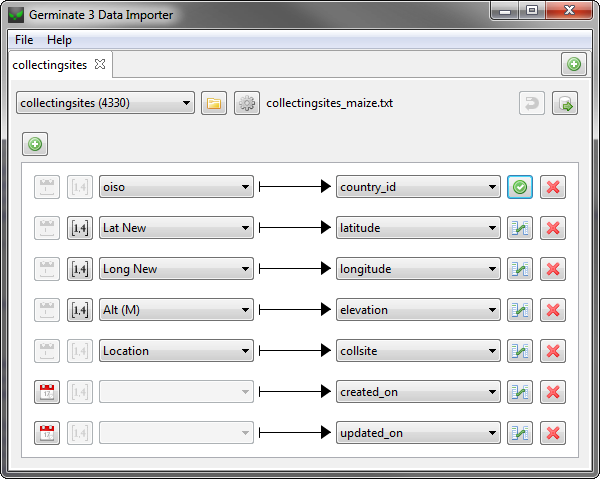
\includegraphics[scale=0.6]{img/import/g3di-mapping.png}
    \caption{Germinate Daim - Column mapping}
    \label{fig:g3di-mapping}
\end{figure}

\noindent Figure \ref{fig:g3di-mapping} shows the main GUI of G3DI with an example mapping. The current tab is used to import data from a text file with the name \texttt{collectingsites\textunderscore maize.txt} into the database table \texttt{collectingsites}. Each row represents a mapping between column of the input file and column of the database. Germinate Daim is aware of the data types of the database columns and provides functionality to accommodate dates, number formats and foreign keys. The first row of the mapping maps \texttt{oiso} (which is a 3-digit country code) to \texttt{country\textunderscore id}. Germinate Daim knows that \texttt{country\textunderscore id} is a foreign key column and requests the user to define a lookup table and column. This lookup is used to find the foreign id based on the value in the \texttt{oiso} column.

As an example, let's assume the lookup table is \texttt{countries} and the lookup column is \texttt{country\textunderscore code3} and the value in the column \texttt{oiso} is "GBR". Germinate Daim will then query the database and determine the id of the country with the 3-digit code "GBR" (which is the United Kingdom) and use this id instead of the actual value.

In addition you can define a number format (or to be exact, a locale) for decimal columns. This format is used to parse your input data before inserting it into the database.

Finally, you can define date formats for columns that represent dates. As an example, let's say your input data is in the form \texttt{dd/MM/yyyy} (2-digit day, 2-digit month, 4-digit year). Germinate Daim will then parse your dates before inserting them into the database. This is necessary, since the database uses its own date format which may differ from the format you used for your data.\\
\\
After you imported your data, you might realize that your mapping was incorrect. Germinate Daim can undo the most recent import step with one click of a button, to allow you to do your work without worrying that you might mess up the database. If you want to be on the safe side, you can still take a backup of the whole database with your favourite database management tool.

\subsection{{\germinate} Data Templates}
Over the years we have learned that people really like Microsoft Excel and that most of the data is stored in Excel spreadsheet before it goes into {\germinate}. To make the best of this fact, we decided to design Excel data templates that specify exactly how your data needs to be formatted for {\germinate} to import it automatically.

The "datatemplates" folder in the {\germinate} source code contains templates for genotypic data, genetic maps, germplasm passport data, pedigree information and trials data. Each of the files contains detailed information about how we require the data to be formatted.

\todo{Explain command line tools}

\subsection{Data Standards}
\todo{fill}
\subsubsection{Dublin Core}
{\germinate} supports the Dublin Core Metadata Element Set \cite{DublinCore} of 15 core terms. These can be associated with a dataset by using the json column \texttt{datasets.dublin\textunderscore core}. Each element of the set is optional, so can either be set to \texttt{null} or left out of it is not required. All elements are arrays, so that multiple values are possible for each key. An example can be seen below:

\begin{lstlisting}[style=JavaScript]
{
	"title": ["An amateur's guide to roasting Unicorns."],
	"subject": ["Unicorns", "Roasting", "Guide"],
	"description": ["Illustrated guide to roasting unicorns. Includes detailed information about the habitat of unicorns and the best way to roast them."],
	"type": ["Text", "Images"],
	"source": ["Deepest depths of a weird mind"],
	"relation": null,
	"coverage": ["2000-2017"],
	"creator": ["Raubach, Sebastian"],
	"publisher": ["The James Hutton Institute"],
	"contributor": null,
	"rights": ["Access limited to everyone except the creator."],
	"date": ["2017-09-28"],
	"format": ["text/plain"],
	"identifier": ["1223-45567-8998"],
	"language": ["English", "German"]
}
\end{lstlisting}
\section{Statistics}
We maintain a Germinate statistics page on our server. It shows an overview of all Germinate instances that we currently maintain. It's available at:
\begin{center}
	\url{http://ics.hutton.ac.uk/germinate/germinate-statistics}
\end{center}
\noindent
Figure \ref{fig:statistics-overview-table} shows one of the visualizations we provide. We're planning to add more visualizations in the future. Now you might think: "What does that have to do with me?".

The answer is simple: We can add your instance of Germinate to our statistics website. That way, people browsing our website may stumble across your site which can broaden your potential target audience. In addition, access to statistical data from more Germinate instances allows us to improve Germinate and the statistics page. So it's basically a win-win situation.\\
\\
If you are interested and want us to add your Germinate instance to our statistics page, or if you have any questions, drop us an email: \url{germinate@hutton.ac.uk}.\\
\\
Just in case you are wondering what kind of data we would collect from your Germinate instance, let me go into detail here: When you start Germinate on your server, it creates a couple of views. These views contain the aggregated data. You can examine these views with your favourite MySQL tool. Let me stress, that these views by themselves are not visible to anyone but you, so there is nothing to worry about.

For us to be able to use these views, you would need to create a new database user that has \texttt{select} and \texttt{show view} privileges on the views. Please note, that this user will not have select access to the database tables, so your actual data is safe. We would then store the user credentials in our database and run a query against your views once a day. Consequently, the data we show on our statistics page is always up to date.

\begin{figure}
	\centering
	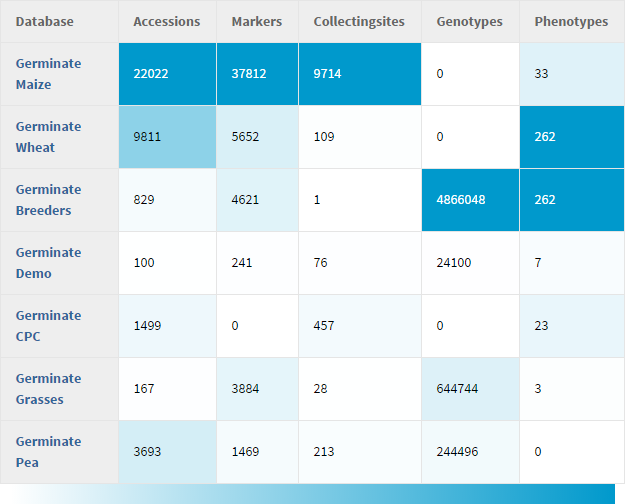
\includegraphics[scale=0.6]{img/statistics/overview-table.png}
	\caption{Statistics overview table}
	\label{fig:statistics-overview-table}
\end{figure}
\section{Troubleshooting}
\label{sec:troubleshooting}

\subsection{Germinate links in download files are not HTTPS}
Files downloaded from Germinate sometimes contain links back to certain pages back on Germinate. This is used so that external tools can come back to Germinate for additional information.

In case you're running Germinate over HTTPS (which you should) and are also using a reverse proxy to forward requests to Tomcat, it might happen that these links don't point to \texttt{https://your-server.com/germinate} but rather to \texttt{http://your-server.com/germinate}. In most cases, this will be fine as the user will be redirected to HTTPS and won't even notice that this happens. Some external tools might not be able to handle this redirect though.

The problem here is that Tomcat doesn't know that the request came to an HTTPS resource originally (before it got proxied) and Germinate therefore doesn't have sufficient information to generate the links correctly.

To fix this, open the \texttt{server.xml} file under Tomcat's \texttt{conf} folder and add the following \texttt{Connector} to the \texttt{Server}:
\begin{lstlisting}[style=Xml]
<Connector port="8081" protocol="HTTP/1.1"
	connectionTimeout="20000"
	proxyName="<proxy server name, e.g. baz.hutton.ac.uk>"
	proxyPort="443"
	scheme="https"
	secure="true"/>
\end{lstlisting}

\noindent
In this case, \texttt{proxyName} is the name of the proxy server. In addition, you need to change the "proxy reverse" settings of Apache. Open the file containing your configuration and identify the entries responsible for Germinate. They may look something like this:

\begin{lstlisting}[style=Proxy]
ProxyPass			/germinate-template http://tomcat-server:8080/germinate-template
ProxyPassReverse	/germinate-template http://tomcat-server:8080/germinate-template
\end{lstlisting}

\noindent
Change the port from 8080 to 8081 (as configured on the \texttt{server.xml}) so that it looks like this:

\begin{lstlisting}[style=Proxy]
ProxyPass			/germinate-template http://tomcat-server:8081/germinate-template
ProxyPassReverse	/germinate-template http://tomcat-server:8081/germinate-template
\end{lstlisting}

\noindent
Restart both Apache and Tomcat for this fix to work.
\section{Funding}
\label{sec:funding}
{\germinate} 3 was developed with CIMMYT \cite{CIMMYT} as part of the MasAgro Seeds of Discovery Project \cite{SeeD}.
\begin{figure}[H]
    \centering
    \vcenteredhbox{
\includegraphics[width=0.16\textwidth]{img/funding/jhi.pdf}}
    \hspace*{0.15cm}
    \vspace*{0.5cm}
    \vcenteredhbox{
\includegraphics[width=0.12\textwidth]{img/funding/cimmyt.pdf}}
    \hspace*{0.15cm}
    \vcenteredhbox{
\includegraphics[width=0.18\textwidth]{img/funding/crop-trust.pdf}}
    \hspace*{0.15cm}
    \vcenteredhbox{
\includegraphics[width=0.12\textwidth]{img/funding/uod.pdf}}
    \hspace*{0.15cm}
	\vcenteredhbox{
\includegraphics[width=0.16\textwidth]{img/funding/bbsrc.pdf}}
	\hspace*{0.15cm}
	\vcenteredhbox{
\includegraphics[width=0.16\textwidth]{img/funding/resas.pdf}}
	\hspace*{0.15cm}
	\vcenteredhbox{
\includegraphics[width=0.10\textwidth]{img/funding/scottish-government.pdf}}
\end{figure}
\section{Technologies}
\label{sec:technologies}
{\germinate} uses third-party software libraries to extend its functionality. The following sections will list these libraries and explain their purpose:

\subsection{JavaScript libraries}

\begin{description}[align=left,style=nextline,leftmargin=*,labelsep=\parindent,font=\bfseries]
	\item[Bootstrap Notify] We use Bootstrap Notify to display notifications on the website.\\\url{https://github.com/mouse0270/bootstrap-notify}
	\item[Bootstrap Switch] Bootstrap Switch makes it easy to use switch or toggle buttons on the web interface.\\\url{https://github.com/Bttstrp/bootstrap-switch}.
	\item[CookieCuttr] Because of the EU "Cookie Law", websites have to let the user know when they're using cookies. CookieCuttr displays a banner notifying the user of just that.\\\url{https://github.com/weare2ndfloor/cookieCuttr}
	\item[D3.js] We us D3.js to generate dynamic and interactive data visualizations. Almost all charts in {\germinate} are created using this library.\\\url{https://github.com/mbostock/d3}
	\item[d3Pie] This is a plugin for D3.js that we use to easily create pie charts.\\\url{https://github.com/benkeen/d3pie}
	\item[D3.tip] This is a plugin for D3.js that allows easy creation of tooltips for SVG elements.\\\url{https://github.com/Caged/d3-tip}
	\item[FancyBox] FancyBox is used to create popups of images and text. \\\url{https://github.com/fancyapps/fancyBox}
	\item[html2canvas] html2canvas is used to convert the d3.js chart legend to an image and download it.
	\\\url{https://github.com/niklasvh/html2canvas}
	\item[jQuery] jQuery is the most popular JavaScript library out there. It allows easy selection, traversal and manipulation of DOM elements. \\\url{https://github.com/jquery/jquery}
	\item[lasso.js]  This is a plugin for D3.js that allows freehand drawing of selections within D3.js charts.\\\url{https://github.com/skokenes/D3-Lasso-Plugin}
	\item[Leaflet] Leaflet is an open-source JavaScript library for mobile-friendly interactive maps. We use it throughout {\germinate} to display data on geographic maps. \\\url{https://github.com/Leaflet/Leaflet}
	\item[prettify.js] Prettify is used to make code on website more pretty, e.g. it adds basic syntax highlighting. The main use of this library is for the SQL debug messages that appear when {\germinate} is run in debug mode.\\\url{https://github.com/google/code-prettify}
	\item[saveSvgAsPng.js] This library allows the user to save a SVG image in the browser (usually generated by D3.js) to a PNG file on their computer.\\\url{https://github.com/exupero/saveSvgAsPng}
	\item[Spectrum] Spectrum allows us to easily add color-pickers to the web-interface. HTML5 introduced the color-type input element, but many current browsers still don't support it. We also always have to consider users with outdated browsers, so unfortunately we have to fall back to a third-party library for this purpose.\\\url{https://github.com/bgrins/spectrum}
\end{description}

\subsection{Web frameworks}
\begin{description}[align=left,style=nextline,leftmargin=*,labelsep=\parindent,font=\bfseries]
	\item[Bootstrap] Bootstrap is one of the most popular web front-end frameworks out there. It provides HTML- and CSS-based templates for interface components and layouts alongside JavaScript extensions for additional functionality.\\\url{https://github.com/twbs/bootstrap}
\end{description}

\subsection{Font frameworks}

\begin{description}[align=left,style=nextline,leftmargin=*,labelsep=\parindent,font=\bfseries]
	\item[Font Awesome] This is a truly awesome framework containing loads of pictographic icons that we use throughout {\germinate}. They are fully scalable which makes them a perfect replacement for raster images. \\\url{https://github.com/FortAwesome/Font-Awesome}
	\item[Material Design Icons] Material Design Icons is an icon set inspired by Google's Material Design guidelines. We use it in addition to Font Awesome within {\germinate}. \\\url{https://github.com/Templarian/MaterialDesign}
\end{description}

\subsection{Java libraries}
\begin{description}[align=left,style=nextline,leftmargin=*,labelsep=\parindent,font=\bfseries]
	\item[Apache Commons CLI] We use this library to easily handle command line parameters for out data import code. \\\url{https://github.com/apache/commons-cli}
	\item[Apache Commons FileUpload] This library is used to make the upload of files from the browser to the server easier. \\\url{https://github.com/apache/commons-fileupload}
	\item[Apache Commons IO] This is a widely used utility library. \\\url{https://github.com/apache/commons-io}
	\item[Apache Commons Logging] A popular logging library. \\\url{https://github.com/apache/commons-logging}
	\item[Apache HttpComponents Client] This library is used to easily communicate with Gatekeeper via HTTP requests. \\\url{https://github.com/apache/httpclient}
	\item[Apache HttpComponents Core] Required by Apache HttpComponents Client. \\\url{https://github.com/apache/httpcore}
	\item[Flapjack] Flapjack is a graphical genotype viewer developed at The James Hutton Institute. {\germinate} uses it on the server side to export genotypic data and allele frequency data. \\\url{https://ics.hutton.ac.uk/flapjack}
	\item[Flyway] Flyway is a database migration tool that {\germinate} uses to update its database between releases.
	\\\url{https://flywaydb.org}
	\item[GWT] GWT is the main building stone of {\germinate}. It's the web development framework we chose to use. \\\url{https://github.com/gwtproject/gwt}
	\item[GWT-Charts] This is a GWT implementation of the JavaScript Google Charts API. \\\url{https://code.google.com/p/gwt-charts}
	\item[GwtQuery] We use this library to use jQuery-like code in Java. \\\url{https://github.com/ArcBees/gwtquery}
	\item[Intro.js] Intro.js is used to display interactive introduction tours that guide the user through a number of steps and explains certain parts of the web interface. \\\url{https://github.com/usablica/intro.js/}
	\item[jBCrypt] jBCrypt is a Java implementation of the OpenBSD's Blowfish password hashing algorithm. \\\url{https://github.com/jeremyh/jBCrypt}
	\item[JAK] This "Java API for KML" is used when exporting geographic information to KML format. \\\url{https://github.com/micromata/javaapiforkml}
	\item[JAXB] Required by JAK.\\\url{https://jaxb.java.net/}
	\item[MySQL Connector/J] This is a library that allows us to easily communicate with a MySQL database from Java code. \\\url{https://github.com/mysql/mysql-connector-j}
	\item[SimpleXML] We use SimpleXML to parse the custom menu of {\germinate} easily. \\\url{https://github.com/ngallagher/simplexml}
	\item[Thumbnailator] This is a utility library used to create thumbnails of images. Whenever a new image is copied to the full-size image folder of {\germinate}, we will use this library to automatically generate a thumbnail for it. \\\url{https://github.com/coobird/thumbnailator}
\end{description}

% add the bubliography (without file extension) and style it
\bibliography{cite}
\bibliographystyle{unsrt}

\end{document}